\chapter[Cooling elastic-plated gravity current]{Elastic-plated gravity current with temperature-dependent
  viscosity}
\label{C3-JFM}

\textit{This Chapter is  part of a paper submitted  for publication to
  Journal  of Fluid  Mechanics (JFM)  untitled: \textbf{Elastic-plated
    gravity current with temperature-dependent viscosity}.}


\minitoc

\begin{abstract}
  Temperature-dependent elastic-plated gravity  currents have numerous
  applications in nature, from shallow magmatic intrusions to the flow
  of melt-water below  an ice sheet. We develop  the general equations
  for an  elastic-plated gravity current with  a temperature-dependent
  viscosity for constant influx conditions.  We show that the coupling
  between  the  thermal  structure  and the  flow  itself  results  in
  important deviations  from the  isoviscous case. In  particular, the
  bending  and  gravity  asymptotic  regimes,  characteristic  of  the
  isoviscous  case,  both  split  into three  phases:  a  first  'hot'
  isoviscous phase, a second phase  where the flow effective viscosity
  and  thickness drastically  increase and  a third  'cold' isoviscous
  phase.   These three  phases are  controlled  by the  extent of  the
  thermal anomaly, for  which we develop analytical  scaling laws. The
  effective flow viscosity  is governed by the local  thermal state at
  the current tip  in the bending regime while it  is the average flow
  viscosity in the gravity regime.  In the end, the complete evolution
  of such  an elastic-plated  gravity current  depends on  its thermal
  state at the transition between  the bending and gravity regimes. We
  provide  a  phase diagram  which  predicts  the different  evolution
  scenarios  as a  function of  the flow  Peclet number  and viscosity
  contrast.

\end{abstract}


\section{Introduction}

Elastic-plated  gravity  currents  involve the  spreading  of  viscous
material beneath  an elastic  sheet. The  applications range  from the
emplacement      of      lava      in      the      shallow      crust
\citep{Michaut:2011kg,Bunger:2011cb} and melt-water drainage below ice
sheet  \citep{Das:2008in,Tsai:2010ev}  in  geological setting  to  the
manufacture of flexible electronics and microelectromechanical systems
(MEMS) in engineering \citep{Hosoi:2004dn}.

When  the thickness  of  the flow  is small  compared  to its  extent,
lubrication  approximation applies  and  the  study of  elastic-plated
gravity currents  resumes to  the study of  a sixth  order, non-linear
partial                      differential                     equation
\citep{Michaut:2011kg,Lister:2013ia,Anonymous:QWXp_4JV}   .   However,
the assumption  that the thickness of  the fluid tends to  zero at the
contact  line  leads  to  divergent viscous  stresses,  and  hence,  a
regularization     condition     is     needed    at     the     front
\citep{Flitton:1999iv,Lister:2013ia,Anonymous:QWXp_4JV}.   One  common
approach is to add a thin  prewetting film of fluid, thus avoiding the
requirement  for   any  boundary   conditions  at  the   contact  line
\citep{Lister:2013ia,Anonymous:QWXp_4JV}.

The dynamics  of the spreading  has been described in  an axisymmetric
geometry   for    a   Newtonian   fluid   with    constant   viscosity
\citep{Michaut:2011kg,Lister:2013ia,Thorey:2014cv}   and    show   two
distinct regimes of  evolution.  First, gravity is  negligible and the
peeling of the front is driven  by bending of the overlying layer; the
interior  is bell-shaped,  the radius  evolves as  $t^{8/22}$ and  the
thickness  as  $t^{7/22}$.   When   the  radius  becomes  larger  than
$4\Lambda$, where  $\Lambda$ is the  flexural wavelength of  the upper
layer, the  weight of  the current becomes  dominant over  the bending
terms    and   the    flow   enters    a   gravity    current   regime
\citep{Huppert:1982a}.  In this regime, the thickness profile develops
a flat top with bent edges,  the radius evolves as $t^{1/2}$ while the
thickness  tends to  a  constant.  Different  analogue experiments  of
isoviscous     flows     confirm     these     theoretical     results
\citep{Dixon:1987js,Lister:2013ia}.

However, in  many real geological settings,  the isothermal/isoviscous
assumption  are not  valid.  For  instance, the  viscosity of  magmas,
produced by partial  melting of the upper mantle, can  vary by several
orders    of   magnitude    \citep{Anonymous:CZVBrBvv,Lejeune:1995fc}.
Therefore,  as the  fluid flows,  it cools  down, its  composition and
crystal content change which, in  turn, modifies the viscosity and the
dynamics of the flow.  Several studies  have shown that, for a gravity
current, this coupling between the cooling and the flow itself results
in     important    deviations     from     the    isoviscous     case
\citep{Bercovici:2007vc,Bercovici:1996uu,BALMFORTH:1999ey,Garel:2014era}.

In  this paper,  we examine  how  the spreading  of an  elastic-plated
gravity current is affected by  the cooling itself.  In particular, we
consider  the  problem  of  an elastic-plated  gravity  current  whose
viscosity depends  on temperature  according to a  prescribed rheology
$\eta(T)$.   This  gives rise  to  a  set  of two  coupled  non-linear
equations  that  we solve  numerically.   We  study the  flow  thermal
structure and its effect on the  dynamics through the rheology in each
regime separately.  In both regimes, we identify different ``thermal''
phases  of  propagation  that  we characterize  by  different  scaling
laws. We  then discuss the  implications of our results  regarding the
evolution with bending and gravity.

\section{Theory}
\label{C3-sec:theory}

\subsection{Formulation}
\label{C3-sec:formulation}

We model  the axisymmetric  flow of  fluid below  an elastic  layer of
constant thickness $d_0$ and above a semi infinite rigid layer (Figure
\ref{C3-Figure2-1}).  The  assumption that the thickness  of the fluid
$h(r,t)$ tends to zero at the  contact line leads to divergent viscous
stresses   and  to   the   theoretical  immobility   of  the   current
\citep{Flitton:1999iv}.   To avoid  problem  at the  contact line,  we
consider    a    thin    prewetting   film    of    thickness    $h_f$
\citep{Lister:2013ia} (Figure \ref{C3-Figure2-1}).

The  fluid is  injected continuously  at the  base and  center of  the
current  at  a constant  rate  $Q_0$  through  a conduit  of  diameter
$a$. The hot fluid is intruded  at temperature $T_i$ and cools through
the  top and  bottom by  conduction in  the surrounding  medium, whose
temperature is  considered constant  and equal to  $T_0$.  In  using a
fixed temperature at the flow boundary, we essentially assume that the
fluid is bounded by a medium with infinite thermal conductivity.

%% FIGURE 2-1
\begin{figure}[h!]
  \begin{center}
    \graphicspath{ {/Users/thorey/Documents/These/Manuscript/Figure/Chapter3/} }
    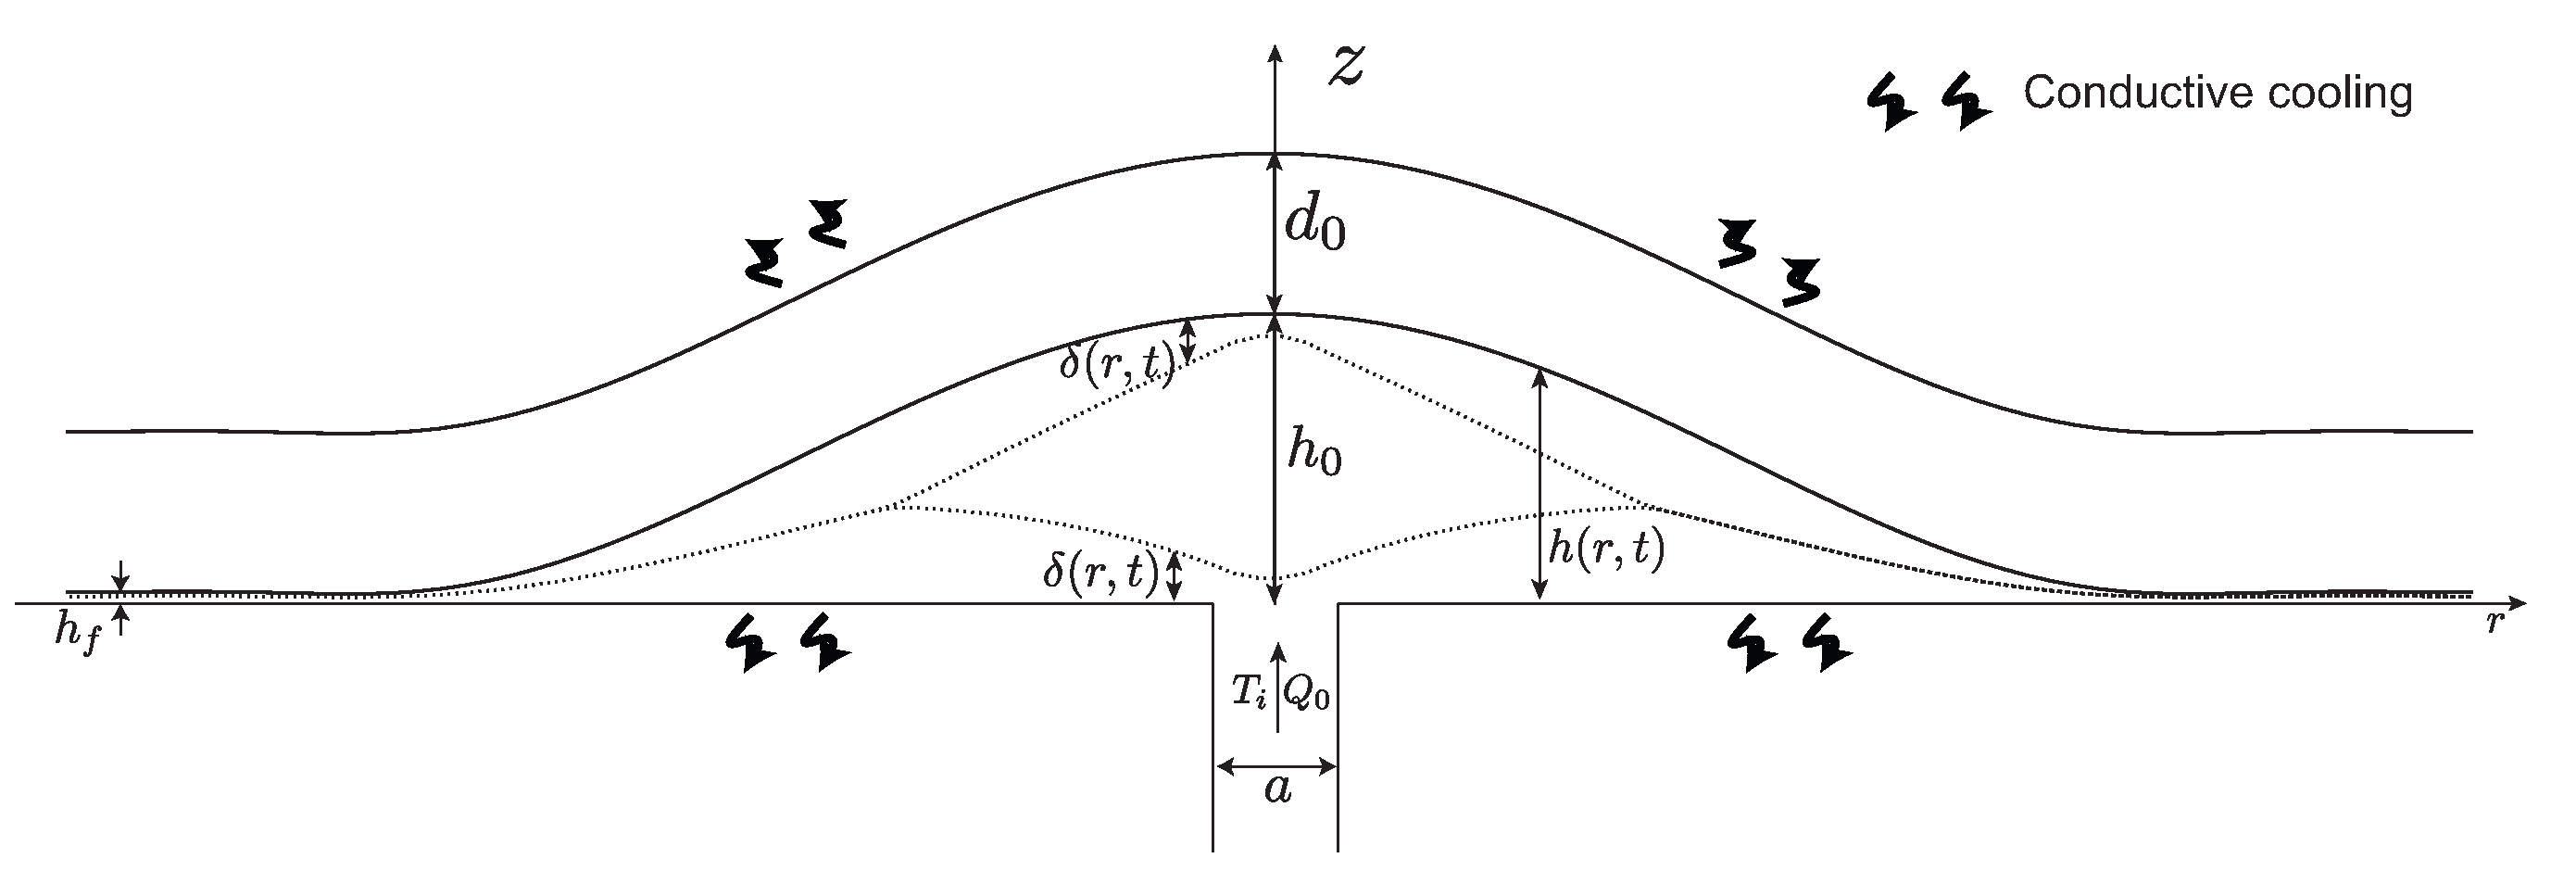
\includegraphics[scale=0.28]{ModelGeometry.eps}
    \caption{Model  geometry and  parameters.  The  vertical scale  is
      exaggerated.}
    \label{C3-Figure2-1}
  \end{center}
\end{figure}

As  it  cools,  the  viscosity  of the  fluid  increases  following  a
prescribed temperature-dependent rheology $\eta(T)$ given by
\begin{equation}
  \eta(T)=\frac{\eta_h
    \eta_c(T_i-T_0)}{\eta_h(T_i-T_0)+(\eta_c-\eta_h)(T-T_0)},
  \label{C3-rheology}
\end{equation}
where $\eta_h$  and $\eta_c$  are the viscosities  of the  hottest and
coldest  fluid  at  the   temperature  $T_i$  and  $T_0$  respectively
\citep{Bercovici:2007vc}.    Although   this   rheology   is   largely
simplified,  the  inverse  dependence   of  viscosity  on  temperature
captures  the  essential  behavior  of  a  viscous  fluid,  i.e.   the
viscosity  variations are  the largest  where the  temperature is  the
coldest
\citep{Anonymous:CZVBrBvv,Marsh:1981dc,Lejeune:1995fc,Giordano:2008em}.

\subsection{Pressure}
\label{C3-sec:Pressure}

The  intrusion develops  over a  length scale  $\Lambda$ that  is much
larger than its thickness $H$ ($H \ll \Lambda$).  In the laminar regime
and  in   axisymmetrical  coordinates  ($r$,$z$),   the  Navier-Stokes
equations within the lubrication approximaton are
\begin{eqnarray}
  -\frac{\partial P}{\partial r}  +  \frac{\partial}{\partial z}\left(\eta(T) \frac{\partial u}{\partial z}\right) &=&0,\label{C3-V1} \\
  -\frac{\partial P}{\partial z}  - \rho_{m}g&  =&0,\label{C3-Npressure}
\end{eqnarray}
where $u(r,z,t)$ is  the radial velocity, $\rho_m$  the fluid density,
$g$  the  standard acceleration  due  to  gravity and  $P(r,z,t)$  the
pressure within the fluid.   Integration of (\ref{C3-Npressure}) gives
the  total pressure  $P(r,z,t)$ within  the flow.   When the  vertical
deflection $h(r,t)$  of the upper  elastic layer is small  compared to
its thickness  $d_0$, i.e $h_0 \ll d_0$,  we can neglect stretching  of the
upper layer and only consider  bending stresses.  Therefore, the total
pressure $P(r,z,t)$ at a level $z$ in  the current is the sum of three
contributions: the weight of the magma  and of the upper layer and the
bending pressure
\begin{equation}
  P = \rho_m g (h-z)+\rho_rgd_0+D_e\nabla_r^4h,
\end{equation}
where  $h(r,t)$ is  the flow  thickness, $\rho_r$  the density  of the
surrounding  rocks and  $D_e$ is  the  flexural rigidity  of the  thin
elastic layer, that depends on  the Young's modulus $E$, the Poisson's
ratio  $\nu^*$   and  on   the  elastic   layer  thickness   $d_0$  as
$D_e = Ed_0^3/\left(12(1-\nu^*)\right)$.

\subsection{Injection rate}

Assuming a Poiseuille flow within the cylindrical feeding conduit, the
vertical injection  velocity $w_i(r,t)$  and injection rate  $Q_0$ are
given by
\begin{equation}
  w_i(r,t)=
  \begin{cases}
    \frac{ \Delta P}{4 \eta_h Z_{c}} (\frac{a^{2}}{4}-r^{2})& r \le \frac{a}{2}\\
    0 & r > \frac{a}{2}
  \end{cases},
  \label{C3-eq12}
\end{equation}
\begin{equation}
  Q_{0}=\frac{\pi \Delta P a^{4}}{128 \eta_h Z_c},
  \label{C3-eq11}
\end{equation}
where  $\Delta P$  is  the  initial overpressure  within  the melt  at
$z=Z_{c}$.

\subsection{Heat transport equation}
\subsubsection*{Local energy conservation}

In the laminar regime and in axisymmetrical coordinates ($r$,$z$), the
local energy  conservation equation within the  lubrication assumption
is
\begin{eqnarray}
  \frac{D}{D t}\left(\rho_m C_{p,m} T+\rho_mL(1-\phi)\right)&=& k_m  \frac{\partial^2
                                                                T}{\partial               z^2},\label{C3-EnergyCons}
\end{eqnarray}
where  $T(r,z,t)$ is  the fluid  temperature and  $\rho_m$, $k_m$  and
$C_{p,m}$ are the  density, thermal conductivity and  specific heat of
the   fluid.   Here,   we   also  account   for   energy  release   by
crystallization of the fluid, which is a non negligible source of heat
for magmas; $\phi(r,z,t)$ is the crystal  fraction in the melt and $L$
the latent heat  of crystallization.  In this model,  the crystals are
considered only  as a source/sink  of energy as they  melt/form during
flow emplacement.  In particular, the physical properties of the fluid
are not modified by the presence of crystals.


Following a common approximation, we  assume that the crystal fraction
is a linear function of temperature over the melting interval
\begin{equation}
  \phi = \frac{T_L-T}{T_L-T_s},
  \label{C3-meltfraction}
\end{equation}
where $T_S$ and $T_L$ are the solidus and liquidus temperatures of the
magma \citep{Hort:1997hk,Michaut:2006di}. In  addition, we assume that
the fluid is  injected at its liquidus temperature ,  i.e. $T_i = T_L$
and, for simplicity, that the surrounding rock temperature is constant
and equal  to the solidus  $T_0 =T_S$. With these  approximations, the
local energy equation (\ref{C3-EnergyCons}) resumes to
\begin{eqnarray}
  \frac{\partial T}{\partial t}+ u\frac{\partial T}{\partial r}
  + w\frac{\partial T}{\partial z}  &=& \frac{ St}{St+1}\kappa_m  \frac{\partial^2
                                        T}{\partial               z^2},
                                        \label{C3-EnergyCons2}
\end{eqnarray}
where  $u(r,z,t)$ and  $w(r,z,t)$ are  the radial  and vertical  fluid
velocities, $St =\left(C_{p,m}(T_i-T_0)\right)/L$ is the Stefan number
and     $\kappa_m$     is     the    fluid     thermal     diffusivity
$\kappa_m = k_m/(\rho_m C_{p,m})$.  We  use an integral balance method
to  solve the  heat transport  equation (\ref{C3-EnergyCons2}).   This
theory is based on the integral-balance method of heat-transfer theory
of  \citet{Goodman:1958ue}, in  which  the vertical  structure of  the
temperature field  is represented  by a known  function of  depth that
approximates the expected solution.

\subsubsection*{Integral   balance   solution   for   the   temperature
  $T(r,z,t)$}

Following \citet{BALMFORTH:1999ey},  we model the cooling  of the flow
through  the  growth  of  two thermal  boundary  layers:  one  growing
downward from the  top and a second growing upward  from the base.  As
we consider homogeneous thermal  properties for the surrounding rocks,
we assume that the two  thermal boundary layers grow symmetrically and
have the same thickness $\delta(r,t)$ (Figure \ref{C3-Figure2-1}).  We
use the  following approximation for the  vertical temperature profile
$T(r,z,t)$
\begin{equation}
  T=
  \begin{cases}
    T_b - (T_b-T_0)(1-\frac{z}{\delta})^2 & 0 \le z\le \delta \\
    T_b & \delta \le z\le h-\delta \\
    T_b - (T_b-T_0)(1-\frac{h-z}{\delta})^2 & h-\delta \le z\le h\\
  \end{cases},
  \label{C3-Temperature}
\end{equation}
where $T_b(r,t)$  is the temperature at  the center of the  flow.  The
integral balance solution in (\ref{C3-Temperature}) assumes a symmetry
around $z=h/2$  and a decrease of  the temperature in the  two thermal
boundary  layers  down  to  the  surrounding  rock  temperature  $T_0$
\citep{BALMFORTH:1999ey}.    In  addition,   it   assumes  a   uniform
temperature  $T_b$ in  between the  thermal boundary  layers.  As  the
fluid is  injected at  temperature $T_i$, we  have $T_b(r,t)  =T_i$ as
long as $\delta<h/2$ (Figure \ref{C3-Figure2-1}).  However, if the two
thermal boundary layers connect, then $\delta = h/2$ and $T_b\le T_i$.
This profile assures  the continuity of the temperature  and heat flux
within the flow.


\subsubsection*{Integral balance equation}
\label{C3-sec:integr-balance-equat}

We  begin  by  integrating  the  local  energy  conservation  equation
(\ref{C3-EnergyCons2})  separately  over   the  two  thermal  boundary
layers.  The integration over the  bottom thermal layer, i.e. from the
base, $z=0$ to a level $z = \delta$ gives
\begin{eqnarray}
  &&\frac{\partial}{\partial t}\left( \delta( \bar{T}-T_b)\right)+\frac{1}{r}\frac{\partial}{\partial r} \left( r\delta(\overline{uT}-\bar{u}T_b)\right) + \delta\left( \frac{\partial T_b}{\partial t}+ \overline{u}\frac{\partial T_b}{\partial r}\right)\nonumber\\
  &=&-\frac{\kappa_m}{1+St}\left. \frac{\partial T}{\partial z}\right|_{z=0}+w_{i}(T_{i}-T_b),
      \label{C3-Local1}
\end{eqnarray}
where the bars  indicate the vertical average over  the bottom thermal
boundary layer
\begin{equation}
  \overline{f} = \frac{1}{\delta}\int_0^{\delta}f dz\nonumber,
\end{equation}
which will be determined once the horizontal flow velocity is derived,
$T_b(r,t)$  is  the  temperature  at  $z=\delta$,  $w_{i}(r)$  is  the
vertical  injection velocity  and  we  have used  the  nullity of  the
thermal gradient at $z=\delta$ and the local mass conservation
\begin{equation}
  \frac{1}{r}\frac{\partial ru}{\partial r} +\frac{\partial w}{\partial z}=0.
  \label{C3-MassConservation}
\end{equation}
The  integration over  the top  thermal layer,  i.e., from  the level,
$z=h-\delta$ to the top $z=h$ gives
\begin{eqnarray}
  &&\frac{\partial}{\partial t}\left( \delta( \bar{T}-T_b)\right)+\frac{1}{r}\frac{\partial}{\partial r} \left( r\delta(\overline{uT}-\bar{u}T_b)\right) + \delta\left(\frac{\partial T_b}{\partial t}+ \overline{u}\frac{\partial T_b}{\partial r}\right)\nonumber\\
  &=&\frac{\kappa_m}{1+St^{-1}}\left. \frac{\partial T}{\partial z}\right|_{z=h},
      \label{C3-Local2}
\end{eqnarray}
where,    in    addition    to    the    local    mass    conservation
(\ref{C3-MassConservation}) and the fact  that the thermal gradient at
$z=h-\delta$ is  equal to  zero, we have  used the  kinematic boundary
condition in $z=h(r,t)$
\begin{equation}
  \frac{\partial h}{\partial t} +u\frac{\partial h}{\partial
    r} = w.
\end{equation}

Therefore,  the  heat  balance   equation,  i.e.   the  heat  equation
(\ref{C3-EnergyCons2}) integrated over the flow thickness, is obtained
by    adding   (\ref{C3-Local1})    and   (\ref{C3-Local2}).     Using
(\ref{C3-Temperature})  to derive  the conductive  fluxes, we  finally
obtain
\begin{eqnarray}
  &&\frac{\partial}{\partial t}\left( \delta( \bar{T}-T_b)\right)+\frac{1}{r}\frac{\partial}{\partial r} \left( r\delta(\overline{uT}-\bar{u}T_b)\right) + \delta\left( \frac{\partial T_b}{\partial t}+ \overline{u}\frac{\partial T_b}{\partial r}\right)\nonumber\\
  &=&-\frac{2\kappa_m}{(1+St^{-1})}\frac{\left( T_b - T_0\right)}{\delta}+\frac{w_{i}}{2}(T_{i}-T_b).
      \label{C3-LocalHeat3}
\end{eqnarray}

\subsection{Equation of motion}
\label{C3-sec:equation-motion}

A global statement of mass conservation gives
\begin{eqnarray}
  \frac{\partial h}{\partial t}+ \frac{1}{r}
  \frac{\partial}{\partial
  r} \left( r\int_0^hudz\right)= w_i.
  \label{C3-C3}
\end{eqnarray}
To obtain an  equation for the flow thickness, we  first note that the
chosen    vertical     structure    of    the     temperature    field
(\ref{C3-Temperature}) is  symmetric around  $h/2$, and  thus, because
the boundary condition are the same  at $z=0$ and $z=h$, the viscosity
and velocity $u$ possess the  same symmetry.  Taking advantage of this
symmetry,      we     integrate      once     (\ref{C3-V1})      using
$\left.\frac{\partial u}{\partial z}\right|_{z=h/2}=0$ to get
\begin{equation}
  \frac{\partial   u}{\partial   z}   =   \frac{1}{\eta(z)}\frac{\partial
    P}{\partial r}\left(z-\frac{h}{2}\right).
  \label{C3-deriv}
\end{equation}
Using no-slip  boundary conditions at  the top  and the bottom  of the
flow, i.e.  $u(r,z=0,t)=u(r,z=h,t)=0$,  (\ref{C3-C3}) can be rewritten
as
\begin{eqnarray}
  \frac{\partial h}{\partial t} = \frac{1}{r}
  \frac{\partial}{\partial
  r} \left( r\int_0^h\frac{\partial u}{\partial z}zdz\right) + w_i.
  \label{C3-Mass}
\end{eqnarray}
Finally,  injecting (\ref{C3-deriv})  into  (\ref{C3-Mass}) gives  the
equation for the flow thickness evolution in axisymmetric coordinates
\begin{eqnarray}
  \frac{\partial h}{\partial t} &=& \frac{1}{r}
  \frac{\partial}{\partial r} \left( r\left(\rho_m g \frac{\partial h}{\partial      r}+D_e\frac{\partial}{\partial      r}\left(\nabla_r^4h\right)\right)\left(\int_0^h\frac{1}{\eta(y)}\left(y-\frac{h}{2}\right)ydy\right)\right)\nonumber\\
  &&+ w_i.
  \label{C3-Mass-2}
\end{eqnarray}
In  addition,  integration  of   (\ref{C3-deriv})  using  the  no-slip
boundary condition at the base of the flow gives
\begin{equation}
  u(r,z,t)        =        \frac{\partial        P}{\partial        r}
  \int_0^z\frac{1}{\eta(y)}\left(y-\frac{h}{2}\right)dy.
  \label{C3-udimensione}
\end{equation}
where
\begin{equation}
  \frac{1}{\eta(y)} = \frac{1}{\eta_c}+\frac{\eta_c-\eta_h}{\eta_h\eta_c}\frac{T(y)-T_0}{T_i-T_0}.
\end{equation}
$T(y)$    being   a    polynomial,   integrals    in   (\ref{C3-Mass-2}),
(\ref{C3-udimensione})   as   well    as   the   averaged   quantities
$\overline{u}$ and $\overline{uT}$ over  the thermal boundary layer in
(\ref{C3-LocalHeat3}) can easily be calculated.

\subsection{Dimensionless equations}
\label{C3-sec:dimens-equat}

We use the characteristic temperature interval $\Delta T = T_i-T_0$ to
nondimensionalize  temperatures.  The  dimensionless integral  balance
approximation (\ref{C3-Temperature}) becomes
\begin{equation}
  \theta=
  \begin{cases}
    \Theta_b\left(1 -(1-\frac{z}{\delta})^2\right)& 0 \le z\le \delta \\
    \Theta_b & \delta \le z\le h-\delta \\
    \Theta_b\left(1-(1-\frac{h-z}{\delta})^2\right)  &   h-\delta  \le
    z\le h
  \end{cases},
  \label{C3-Temperature2}
\end{equation}
where   $\theta(r,z,t)$   is   the   dimensionless   temperature   and
$\Theta_b=\frac{T_b-T_0}{T_{i}-T_0}$.         Finally,       equations
(\ref{C3-LocalHeat3})  and  (\ref{C3-Mass-2})  are  nondimensionalized
using a  horizontal scale $\Lambda$, a  vertical scale $H$ and  a time
scale $\tau$ given by
\begin{eqnarray}
  \Lambda &=& \left(\frac{D_e}{\rho_m g}\right)^{1/4}\label{C3-L1},\\
  H&=&\left       (\frac{12\eta_h      Q_{0}}{\rho_{m}g       \pi}\right      )
       ^{1/4} \label{C3-H1},\\
  \tau&=&\frac{\pi \Lambda^{2} H}{Q_{0}}\label{C3-T1},
\end{eqnarray}
where  $\Lambda$  represents  the  flexural wavelength  of  the  upper
elastic layer \citep{Michaut:2011kg}, $H$ the characteristic thickness
of an isoviscous constant flux gravity current with viscosity $\eta_h$
\citep{Huppert:1982wr} and $\tau$ the characteristic time to fill up a
cylindrical flow of  radius $\Lambda$ and thickness $H$  at a constant
rate $Q_0$.   In addition, we  can define a horizontal  velocity scale
$U=\Lambda/\tau=\left(\rho_m           g           H^3\right)/\left(12
  \eta_h\Lambda\right)$ and a pressure scale $\rho_m g H$.

The dimensionless equations are
\begin{eqnarray}
  \frac{\partial h}{\partial t}& =& \frac{12}{r}
                                    \frac{\partial}{\partial r} \left( r\left( \frac{\partial h}{\partial      r}+\frac{\partial}{\partial      r}\left(\nabla_r^4h\right)\right)I_1(h)\right)
                                    + w_i\label{C3-EqFinal1},\\
  \frac{\partial}{\partial
  t}\left( \delta( \bar{\theta}-\Theta_b)\right)&=&-\frac{1}{r}\frac{\partial}{\partial
                                                    r}  \left(   r\delta(\overline{u\theta}-\bar{u}\Theta_b)\right)  -
                                                    \delta\left(      \frac{\partial       \Theta_b}{\partial      t}+
                                                    \overline{u}\frac{\partial     \Theta_b}{\partial    r}\right)\nonumber\\
                               &-&
                                   2Pe^{-1}St_m\frac{\Theta_b}{\delta}+\frac{w_{i}}{2}(1-\Theta_b)\label{C3-HeatDimensionLess},\\
  w_{i}&=&\mathcal{H}(\frac{\gamma}{2}-r)
           \frac{32}{\gamma^{2}}\left(\frac{1}{4}-\frac{r^{2}}{\gamma^{2}}\right),\\
  u(r,z,t)&   =&   12\left(   \frac{\partial   h}{\partial
                 r}+\frac{\partial}{\partial
                 r}\left(\nabla_r^4h\right)\right)I_0(z)\label{C3-Veloc},
\end{eqnarray}
with
\begin{eqnarray}
  I_0(z)&=&\int_0^z \left(\nu+(1-\nu)\theta(y)\right)\left(y-\frac{h}{2}\right)
            dy \label{C3-I_1},\\
  I_1(z) &=& \int_0^z \left(\nu+(1-\nu)\theta(y)\right)\left(y-\frac{h}{2}\right)y dy\label{C3-I_2}.
\end{eqnarray}
$\mathcal{H}$ is the Heaviside function and $\gamma$, $Pe$, $St_m$ and
$\nu$ are the four dimensionless  numbers that control the dynamics of
the flow
\begin{eqnarray}
  \gamma&=&\frac{a}{\Lambda} \label{C3-gamma},\\
  Pe&=&            \frac{H^2}{\kappa_m            \tau}\label{C3-Pe},\\
  St_m &=& \frac{C_{p,m}\left(T_i-T_0\right)}{C_{p,m}\left(T_i-T_0\right)+L} \label{C3-St},\\
  \nu&=& \frac{\eta_h}{\eta_c}\label{C3-nu}.
\end{eqnarray}
$\gamma$  is the  dimensionless radius  of  the conduit,  it does  not
significantly influence  the flow and is  set to $0.02$ in  this study
\citep{Michaut:2009jx,Michaut:2011kg}; $Pe$ is the Peclet number which
compares the vertical diffusion of heat to the horizontal advection in
the interior; $St_m$ is a  modified Stefan number which represents the
ratio  of sensible  heat between  solidus  and liquidus  to the  total
energy  of the  fluid at  the liquidus  temperature and  $\nu$ is  the
maximum viscosity  contrast, i.e.  the  ratio between the  hottest and
coldest viscosity.

\subsection{Further simplifications}
\label{C3-sec:furth-simpl}

\subsubsection{Heat equation}
\label{C3-sec:heat-equation}

In the end, the heat balance equation (\ref{C3-HeatDimensionLess}) can
reduce to
\begin{eqnarray}
  \frac{\partial}{\partial
  t}\left( \delta( \bar{\theta}-1)\right)+\frac{1}{r}\frac{\partial}{\partial
  r}
  \left( r\delta(\overline{u\theta}-\bar{u})\right)&=&- 2Pe^{-1}St_m\frac{\Theta_b}{\delta}.
                                                       \label{C3-HeatD_a}
\end{eqnarray}
Indeed, if  the thermal boundary layers  exist, $\Theta_b=1$, $\delta$
is  the variable  quantity  and (\ref{C3-HeatDimensionLess})  directly
reduces to  (\ref{C3-HeatD_a}).  In contrast, if  the thermal boundary
layers merge,  $\delta=h/2$ and  the variable quantity  is $\Theta_b$.
In this  case, the heat balance  equation (\ref{C3-HeatDimensionLess})
reduces to
\begin{eqnarray}
  \frac{\partial h\bar{\theta}}{\partial t}+\frac{1}{r}\frac{\partial}{\partial
  r} \left( rh\overline{u\theta}\right)-\Theta_b\left(\frac{\partial h}{\partial t}+\frac{1}{r}\frac{\partial}{\partial
  r}           \left(           rh\bar{u}\right)\right)&=&           -
                                       8St_mPe^{-1}\frac{\Theta_b}{h}\nonumber\\
&&+w_{i}(1-\Theta_b),
\end{eqnarray}
which, by using (\ref{C3-C3}), rewrites
\begin{equation}
  \frac{\partial h\bar{\theta}}{\partial t}+\frac{1}{r}\frac{\partial}{\partial
    r} \left( rh\overline{u\theta}\right) &=& w_i
  - 8St_mPe^{-1}\frac{\Theta_b}{h}.
  \label{C3-eqHS2}
\end{equation}
Equation (\ref{C3-eqHS2}) also  corresponds to (\ref{C3-HeatD_a}) when
$\delta=h/2$.

Following  \citet{BALMFORTH:1999ey},   we  rewrite  (\ref{C3-HeatD_a})
using a new variable $\xi = \delta(1-\overline{\theta})$
\begin{equation}
  \frac{\partial \xi}{\partial t}+\frac{1}{r}\frac{\partial}{\partial r} \left( r\bar{u}\xi\right)-\frac{1}{r}\frac{\partial}{\partial r} \left( r\delta(\overline{u\theta}-\bar{u}\bar{\theta})\right)&=&2Pe^{-1}St_m\frac{\Theta_b}{\delta},
  \label{C3-EqFinal2}
\end{equation}
where our  unknown $\Theta_b$ or  $\delta$ can be  calculated directly
from  the expression  of  $\xi$ using  $\delta  =h/2$ or  $\Theta_b=1$
respectively

\begin{tabular}{p{6cm}p{6cm}}
{
\begin{equation}
    \Theta_b(r)=
    \begin{cases}
      1 &\text{if } \hspace{.5cm} \xi\leq \xi_t \nonumber\\
      \frac{3}{2}-\frac{3\xi}{h} & \text{if} \hspace{.5cm} \xi > \xi_t\nonumber
    \end{cases},
  \end{equation}
                                   }
&
{
  \begin{equation}
    \delta(r)=
    \begin{cases}
      3\xi &\text{if } \hspace{.5cm} \xi\leq \xi_t \nonumber\\
      h(r,t)/2 & \text{if} \hspace{.5cm} \xi > \xi_t\nonumber\\
    \end{cases},
  \end{equation}
  }
\end{tabular}
with $\xi_t = h/6$.

The second term on the  left hand side of (\ref{C3-EqFinal2}) contains
advection by the vertically integrated radial velocity while the third
term contains  a correction accounting  for the vertical  structure of
the temperature field.  The  term on the right is the  loss of heat by
conduction in the surrounding medium.

\subsubsection{Average quantities}
The  average velocity  over  a thermal  boundary layer  $\overline{u}$
reads
\begin{eqnarray}
  \overline{u}        =\frac{1}{\delta}\int_0^{\delta}u dz        &=&
                                                                     u(r,\delta,t) - \frac{1}{\delta}\int_0^{\delta}\frac{\partial
                                                                     u}{\partial
                                                                     z}
                                                                     zdz\label{C3-eqHello}\\
                                                                 &=&\frac{12}{\delta}
                                                                     \frac{\partial
                                                                     P}{\partial
                                                                     r}\left(\delta
                                                                     I_0(\delta)-I_1(\delta)\right),
\end{eqnarray}
where $P(r,z,t) = h+\nabla_r^4h$ is the dimensionless dynamic pressure
and we have used  (\ref{C3-deriv}) in (\ref{C3-eqHello}).  The average
rate  of heat  advected $\overline{u\theta}$  over a  thermal boundary
layer reads
\begin{eqnarray}
  \overline{u\theta}=\frac{1}{\delta}\int_0^{\delta}u\theta dz &=& \frac{1}{\delta}\left( [ uG(z) ]_{0}^{\delta} -\int_0^\delta
                                                                   G(z)\frac{\partial
                                                                   u}{\partial
                                                                   z}
                                                                   dz\right)\nonumber\\
                                                               &=&\frac{12}{\delta} \frac{\partial P}{\partial r}\left(G(\delta)I_0(\delta)-I_2(\delta)\right),
\end{eqnarray}
where
\begin{equation}
  G(z)= \frac{\Theta_{b} z^{2}}{3 \delta^{2}} \left( 3 \delta - z\right)
\end{equation}
is a primitive of $\theta$ when $z<\delta$ and
\begin{equation}
  I_2(z)=\int_0^z\left(\nu+(1-\nu)\theta(y)\right)G(y)
  \left(y-\frac{h}{2}\right)dy.
  \label{C3-I_3}
\end{equation}
Therefore, we have
\begin{equation}
  \overline{u\theta}-\overline{u}\overline{\theta}= \frac{12}{\delta} \frac{\partial P}{\partial r}\left(I_0(\delta)\left(G(\delta)-\delta\overline{\theta}\right)+\overline{\theta}I_1(\delta)-I_2(\delta)\right),
\end{equation} 
where  the  average  temperature  over a  thermal  boundary  layer  is
$ \overline{\theta} = 2\Theta_{b}/3$.

\subsection{Summary of the equations}
\label{C3-sec:summary-equations}

In  the  end,  the  coupled  equations governing  the  cooling  of  an
elastic-plated gravity current are
\begin{eqnarray}
  \frac{\partial h}{\partial t}-\frac{12}{r}
  \frac{\partial}{\partial      r}
  \left( r I_1(h) \frac{\partial P}{\partial
  r}\right)
  \label{C3-HF}
  & =& \mathcal{H}(\frac{\gamma}{2}-r)\frac{32}{\gamma^{2}}\left(\frac{1}{4}-\frac{r^{2}}{\gamma^{2}}\right),\\
  \frac{\partial                                       \xi}{\partial
  t}+\frac{1}{r}\frac{\partial}{\partial                          r}
  \left( r\left(\bar{u}\xi-\Sigma\right)\right)&=&2Pe^{-1}St_m\frac{\Theta_b}{\delta},\label{C3-TF}
\end{eqnarray}
with

\begin{tabular}{p{6cm}p{6cm}}
{
\begin{equation}
    \Theta_b(r)=
    \begin{cases}
      1 &\text{if } \hspace{.5cm} \xi\leq \xi_t \nonumber\\
      \frac{3}{2}-\frac{3\xi}{h} & \text{if} \hspace{.5cm} \xi > \xi_t\nonumber
    \end{cases},
  \end{equation}
                                   }
&
{
  \begin{equation}
    \delta(r)=
    \begin{cases}
      3\xi &\text{if } \hspace{.5cm} \xi\leq \xi_t\\
      h(r,t)/2 & \text{if} \hspace{.5cm} \xi > \xi_t\nonumber\\
    \end{cases},
  \end{equation}
  }
\end{tabular}
\begin{eqnarray}
  \overline{u}&=& \frac{12}{\delta}\frac{\partial P}{\partial r}\left(\delta
                  I_0(\delta)-I_1(\delta)\right) \label{C3-ubarF},\\
  \Sigma     &=& \frac{\partial     P}{\partial
                 r}\left(8I_1(\delta)\Theta_b-12I_2(\delta)\right),\label{C3-SigmaF}
\end{eqnarray}
where  $P   =  h+\nabla_r^4h$   is  the  dimensionless   pressure  and
$\mathcal{H}$   the    Heaviside   function.    The    expression   of
$I_0(\delta)$, $I_1(h)$,  $I_1(\delta)$ and  $I_2(\delta)$ as  well as
the  numerical  scheme  used  to  solve  equations  (\ref{C3-HF})  and
(\ref{C3-TF}) are given in Appendix \ref{A1-sec:-cool-elast-plat}.

\subsection{Preliminary results for an isothermal flow}
\label{C3-sec:prel-results-isoth}

For a constant injection rate, a small prewetting film thickness, i.e.
$h_f \ll 1$  and  a  viscosity  contrast   $\nu$  set  to  1,  numerical
resolution  of (\ref{C3-HF})  shows two  asymptotic spreading  regimes
\citep{Michaut:2011kg,Lister:2013ia}.
\begin{figure}[h!]
  \begin{center}
    \graphicspath{ {/Users/thorey/Documents/These/Projet/Refroidissement/Skin_Model/Figure/JFM_V13/} }
    \includegraphics[scale=0.45]{Scaling_HR_ELASGRAV_Simple.eps}
    \caption{Left: Dimensionless thickness at  the center $h_0$ versus
      dimensionless  time  $t$.   Dotted-lines: scaling  laws  in  the
      bending regime $h_0= 0.7h_f^{-1/11}t^{8/22}$  and in the gravity
      regime where  $h_0$ tends  to a constant.   Right: Dimensionless
      radius $R$ versus dimensionless time $t$.  Dotted-lines: scaling
      laws in the bending regime $R= 2.2h_f^{1/22}t^{7/22}$ and in the
      gravity current regime $R\propto t^{1/2}$.}
    \label{C3-Scaling_HR_ELASGRAV_Simple}
  \end{center}
\end{figure}

At  early times,  when $R \ll \Lambda$,  gravity is  negligible and  the
spreading dynamics is governed by the bending of the upper layer.  The
spreading  is  very  slow  and   the  interior  has  uniform  pressure
$P =\nabla_r^4h$.  The flow is  bell-shaped and its thickness is given
by
\begin{equation}
  h(r,t) = h_0(t)\left(1-\frac{r^2}{R^2(t)}\right)^2,
  \label{C3-IntrusionShape}
\end{equation}
with   $h_0(t)$  the   thickness  of   the  current   at  the   center
\citep{Michaut:2011kg,Lister:2013ia}.       In       this      regime,
\citet{Lister:2013ia} have  shown that the spreading  is controlled by
the propagation  of a peeling by  bending wave at the  flow front with
dimensionless velocity $c$
\begin{equation}
  c=    \frac{d             R}{d            t}             =h_f^{1/2}
  \left(\frac{\kappa}{1.35}\right)^{5/2},
  \label{C3-WaveVelocity}
\end{equation}
where  $\kappa  =  \partial^2  h/\partial r^2$  is  the  dimensionless
curvature  of  the  interior  solution.   Using  the  propagation  law
(\ref{C3-WaveVelocity})  and   the  form  of  the   interior  solution
(\ref{C3-IntrusionShape}),  \citet{Lister:2013ia}  predicted that,  in
this regime, the flow radius and height evolve following
\begin{eqnarray}
  h_0(t)&=& 0.7 h_f^{-1/11}t^{8/22}\label{C3-ScalingH},\\
  R(t) &=& 2.2h_f^{1/22}t^{7/22}\label{C3-ScalingR},
\end{eqnarray}
where the numerical pre-factor obtained in our simulations match those
of \citet{Lister:2013ia} (Figure \ref{C3-Scaling_HR_ELASGRAV_Simple}).

In  contrast,  when  the  radius  R  becomes  larger  than  $4\Lambda$
($R>>\Lambda$), the  weight of the  current becomes dominant  over the
bending  terms.  The  pressure is  given by  the hydrostatic  pressure
$P =  h$ and  the current  enters a  classical gravity  current regime
where bending  terms only  affect the  solution near  the edge  of the
current  \citep{Huppert:1982a,Michaut:2011kg,Lister:2013ia}.  In  this
second regime, the radius evolves as $t^{1/2}$ and the thickness tends
to a constant (Figure \ref{C3-Scaling_HR_ELASGRAV_Simple}).

In  the following,  we study  the effect  of the  cooling on  the flow
dynamics in  both regimes  separately. We  first describe  the thermal
structure  for an  isoviscous flow,  i.e. $\nu=1$  and then  study the
effect  of the  temperature-dependent viscosity  on the  flow dynamics
without  crystallization,  i.e  $St_m   =1$.   Finally,  we  introduce
crystallization by  setting $St_m<1$.  For simplicity,  we present the
results for  a given  film thickness ($h_f=5\times  10^{-3}$); results
for different film thicknesses are shown in Appendix \ref{chap:A3}.

\section{Evolution in the bending regime}
\label{C3-sec:evol-bend-regime}

We first concentrate on the case  in which only bending contributes to
the dynamic pressure.  The  governing equations are thus (\ref{C3-HF})
and (\ref{C3-TF}) where $P=\nabla_r^4h$.

\subsection{Thermal structure for an isoviscous flow, effect of $Pe$}
\label{C3-sec:thermal-structure-an}

The current  cools by conduction  and thermal boundary layers  form at
the contact with the surrounding  medium.  These boundary layers first
connect at the  tip of the flow, where the  small thickness induces an
important cooling (Figure \ref{C3-Grid_Time_ELAS}).   A region of cold
fluid forms at the front.

As the  current thickens  with time, a  balance between  advection and
diffusion of heat is never reached in the interior of the current. The
hot thermal  anomaly grows  in extent  with time  but slower  than the
current  itself and  the  cold fluid  region at  the  tip grows.   For
instance, for $Pe  =100$, while the region of cold  fluid extends over
about $10\%$ of  the current at $t=0.5$, it extends  over about $20\%$
at $t =10$ (Figure \ref{C3-Grid_Time_ELAS}).  

The smaller  $Pe$, the more  important the conductive cooling  and the
larger   the   cold   region   (Figure   \ref{C3-Grid_PeNu_ELAS}   and
\ref{C3-Thickness_Temperature_Profile_ELAS}).    For    instance,   at
$t=10$, while the cold region extends over about $20\%$ of the current
for  $Pe=100$, it  extends over  more than  $70\%$ for  $Pe=1$ (Figure
\ref{C3-Grid_PeNu_ELAS}).

\begin{figure}[h!]
  \begin{center}
    \graphicspath{ {/Users/thorey/Documents/These/Projet/Refroidissement/Skin_Model/Figure/JFM_V13/} }
    \includegraphics[scale=0.35]{Grid_Time_ELAS_Pe1_Nu1.eps}
    \caption{Snapshots of  the flow thermal  structure $\theta(r,z,t)$
      at  different  times  indicated   on  the  plot.   Dashed  lines
      represent  the thermal  boundary  layers. Solid  grey lines  are
      isotherms for  $\theta =  0.2$, $0.4$,  $0.6$ and  $0.8$.  Here,
      $\nu=1.0$, $Pe =100$, $St_m = 1$.}
    \label{C3-Grid_Time_ELAS}
  \end{center}
\end{figure}

\begin{figure}[h!]
  \begin{center}
    \graphicspath{ {/Users/thorey/Documents/These/Projet/Refroidissement/Skin_Model/Figure/JFM_V13/} }
    \includegraphics[scale=0.48]{Grid_PeNu_ELAS_Final_2.eps}
    \caption{Snapshots of  the flow thermal  structure $\theta(r,z,t)$
      for different sets ($\nu$,$Pe$) with $\nu= 1$, $0.1$, $0.01$ and
      $0.001$ and  $Pe=1$, $10$,  $100$ and  $1000$ at  $t=10$.  While
      $Pe$ controls the  thermal structure of the flow, it  has only a
      small influence on the flow  aspect ratio which is controlled by
      $\nu$.}
    \label{C3-Grid_PeNu_ELAS}
  \end{center}
\end{figure}

\begin{figure}[h!]
  \begin{center}
    \graphicspath{ {/Users/thorey/Documents/These/Projet/Refroidissement/Skin_Model/Figure/JFM_V13/} }
    \includegraphics[scale=0.4]{Thickness_Temperature_Profile_ELAS.eps}
    \caption{Left: thickness normalized by the thickness at the center
      $h(r,t)/h_0(t)$  versus radial  axis normalized  by the  current
      radius $r/R(t)$  at different  times indicated  on the  plot for
      $Pe=1.0$  and $\nu=1.0$.   Solid-lines  represent the  thickness
      profiles.  Dashed-lines  represent the thermal  boundary layers.
      Right: Same plot but for $\nu=10^{-3}$.}
    \label{C3-Thickness_Temperature_Profile_ELAS}
  \end{center}
\end{figure}



\subsection{Thickness and temperature profile, effect of $\nu$}
\label{C3-sec:thickn-temp-prof-1-e}

When accounting for  the temperature dependence of  the viscosity, the
region of cold  fluid at the tip  is marked by a  higher viscosity and
enhances flow thickening at the  expense of spreading.  The larger the
viscosity  contrast,  the  larger  the aspect  ratio  $h_0/R$  (Figure
\ref{C3-Grid_PeNu_ELAS}).  For instance, for the same value of $Pe=1$,
while the aspect ratio is $0.7$ for  $\nu=1$ at $t=10$, it is $4.2$ at
the  same  time  for $\nu=10^{-3}$  (Figure  \ref{C3-Grid_PeNu_ELAS}).
Nevertheless, the shape of  the flow remains essentially self-similar,
i.e.  well  described  by   (\ref{C3-IntrusionShape})  and  cannot  be
differentiated  from  the  shape  of  an  isoviscous  current  if  the
thickness and the radial coordinates  are rescaled by the thickness at
the     center     $h_0(t)$      and     radius     $R(t)$     (Figure
\ref{C3-Thickness_Temperature_Profile_ELAS}).

The flow thermal  structure is similar to the  isoviscous case (Figure
\ref{C3-Grid_PeNu_ELAS}),  the thermal  anomaly rapidly  detaches from
the tip  of the  current and a  region of cold  fluid develops  at the
front  where  heat  loss  is  the  largest.   However,  the  important
thickening induced by  the viscosity increase limits heat  loss to the
surrounding.   The  larger  the  viscosity contrast  $\nu$,  the  more
important the thickening and the larger the thermal anomaly at a given
time.  For  instance, for  $Pe=1$, while  the thermal  anomaly extends
over about $30\%$  of the flow for $\nu=1$ at  $t=10$, it extends over
more than $50\%$ for $\nu=10^{-3}$ (Figure \ref{C3-Grid_PeNu_ELAS}).

As expected, a larger Peclet number  leads to a larger thermal anomaly
(Figure \ref{C3-Grid_PeNu_ELAS}).  However,  although different Peclet
numbers cause very different thermal  structures, the influence of the
Peclet number on  the flow morphology is small, much  smaller than the
effect     of     the     viscosity     contrast     $\nu$     (Figure
\ref{C3-Grid_PeNu_ELAS}).  For instance,  for $\nu=10^{-3}$ at $t=10$,
the thermal  anomaly is still attached  to the tip of  the current for
$Pe = 1000$  whereas it makes about $50\%$ of  the current for $Pe=1$;
but, the thickness $h_0$ and the  radius $R$ in both cases differ only
by  a few  percents (Figure  \ref{C3-Grid_PeNu_ELAS}).  This  suggests
that, in this  regime, the spreading of the flow  is not controlled by
the mean temperature or average viscosity of the flow.
  
\subsection{Evolution of the thickness and the radius}
\label{C3-sec:evol-thickn-radi-e}

In this bending  dominated regime, the dynamics  shows three different
spreading phases.   The thickness as  well as the radius  first follow
the   isoviscous   scaling   laws   for  a   hot   viscosity   current
$h_0\propto  t^{8/22}$  (\ref{C3-ScalingH})  and  $R\propto  t^{7/22}$
(\ref{C3-ScalingR}) (Figure \ref{C3-Scaling_HR_ELAS}).   In the second
phase,  thickening occurs  at  the expense  of  spreading because  the
thermal anomaly has  detached from the current radius  and the viscous
cold fluid region at the front slows down the spreading.  Finally, the
dynamics enters  a third phase  where the thickness and  radius follow
the  scaling  laws   for  the  spreading  of   an  isoviscous  current
characterized by a dimensionless cold viscosity $1/\nu$. These scaling
laws are obtained from  (\ref{C3-ScalingH}) and (\ref{C3-ScalingR}) by
rescaling  the characteristic  thickness and  time by  $\nu^{1/4}$ and
read
\begin{eqnarray}
  h_{0} & = &0.7 \nu^{-2/11} h_f^{-1/11}t^{8/22}\label{C3-ScalingH-Visco},\\
  R& = & 2.2 \nu^{1/11}h_f^{1/22} t^{7/22}\label{C3-ScalingR-Visco}.
\end{eqnarray}
\begin{figure}[h!]
  \begin{center}
    \graphicspath{ {/Users/thorey/Documents/These/Projet/Refroidissement/Skin_Model/Figure/JFM_V13/} }
    \includegraphics[scale=0.45]{Scaling_HR_ELAS.eps}
    \caption{Left: Dimensionless thickness at  the center $h_0$ versus
      dimensionless time  $t$ for different sets  $(\nu,Pe)$ indicated
      on      the      plot.      Dotted-lines:      scaling      laws
      $h_0=  0.7h_f^{-1/11}\nu^{-2/11}t^{8/22}$ for  $\nu  = 1.0$  and
      $0.001$.  Right:  Dimensionless radius $R$  versus dimensionless
      time $t$ for the same  sets of values $(\nu,Pe)$.  Dotted-lines:
      scaling    laws    $R=   2.2h_f^{1/22}\nu^{1/11}t^{7/22}$    for
      $\nu = 1.0$ and $0.001$.}
    \label{C3-Scaling_HR_ELAS}
  \end{center}
\end{figure}
The dependence on  the viscosity contrast $\nu$ indeed  fits very well
the  third phase  of the  flow observed  in the  numerical simulations
(Figure   \ref{C3-Scaling_HR_ELAS}).   In   the  end,   the  effective
viscosity $\eta_e$ of  the flow evolves from the viscosity  of the hot
fluid in the first phase to asymptotically tend to the one of the cold
fluid in the third phase.

The time  the flow spends in  each phase depends on  the Peclet number
$Pe$.  For instance,  for $\nu=10^{-3}$, while the  current leaves the
first phase at $t \sim 10^{-6}$ for $Pe =1.0$, this transition happens
only   after   $t   \sim   10^{-2}$    for   $Pe   =   10^3$   (Figure
\ref{C3-Scaling_HR_ELAS}).   The larger  the Peclet  number, the  less
efficient the  cooling and  thus the  longer the  flow remains  in the
first phase and the later it reaches the third phase.

\subsection{Characterization of the thermal anomaly}
\label{C3-sec:char-therm-anom-e}

Following \citet{Garel:2012bh},  we quantify  the size of  the thermal
anomaly  through   a  critical  thermal  radius   $R_c(t)$  where  the
temperature  at the  center of  the flow  $\Theta_b$ is  $1\%$ of  the
injection temperature,  i.e.  $\Theta_b(r=0)-\Theta_b(r=R_c)  = 0.99$.
The thermal  anomaly is  first advected  at the  same velocity  as the
current  itself,  i.e.   $R(t) =  R_c(t)$  (Figure  \ref{C3-R_Rc_ELAS}
left).   After a  time that  depends on  $Pe$ and  $\nu$, the  thermal
anomaly detaches  from the tip  and $R(t)-R_c(t)$ increases  with time
(Figure \ref{C3-R_Rc_ELAS}) .

In  the bending  regime, the  interior  pressure is  constant and  the
thickness profile $h(r)$ is given by (\ref{C3-IntrusionShape}) (Figure
\ref{C3-Thickness_Temperature_Profile_ELAS}).   The time  evolution of
the size of  the thermal anomaly $R_c(t)$ is  characterized by looking
at the radius  in the flow where heat advection  locally balances heat
loss, i.e.
\begin{eqnarray}
  \frac{d}{dt}\left(\Theta_bh\right)&\approx& Pe^{-1}
                                              \frac{\Theta_b}{h}\label{C3-Calcul1}.
\end{eqnarray}
Using     the     thickness     profile     (\ref{C3-IntrusionShape}),
(\ref{C3-Calcul1}) becomes
\begin{eqnarray}
  \alpha^2\left(1+\frac{R_c}{R}\right)^2\left(\Theta_b\frac{d h_0}{d
  t}+h_0\frac{d \Theta_b}{d
  t}\right)+\frac{4h_0R_c^2\Theta_b}{R^3}\frac{d
  R}{d
  t}\alpha\left(1+\frac{R_c}{R}\right) \approx \frac{Pe^{-1}\Theta_b}{\alpha^2\left(1+\frac{R_c}{R}\right)^2h_0},\nonumber
\end{eqnarray}
where  $\alpha (t)=  \left(R(t)-R_c(t)\right)/R(t)$ is  the normalized
region   beyond   $r=R_c(t)$.    In  the   limit   $\alpha \ll 1$,   i.e.
$R_c/R\sim  1$,  the  time  derivative is  locally  dominated  by  its
advective part ($\propto \alpha$) and we finally get
\begin{equation}
  \alpha^3\approx \frac{Pe^{-1}} {h_0^2(t)}\frac{R}{\frac{\partial R}{\partial t}}.
\end{equation}
Substituting  $h_0(t)$ and  $R(t)$  by their  respective scaling  laws
(\ref{C3-ScalingH-Visco})  and   (\ref{C3-ScalingR-Visco}),  the  size
evolution of the normalized cold front region $\alpha$ reads
\begin{equation}
  \alpha(t)&\approx& Pe^{-1/3}\nu^{4/33} h_f^{2/33}t^{1/11},
  \label{C3-ScalingXi}
\end{equation}
which is equivalent to
\begin{equation}
  R(t)-R_c(t) = 2.1 Pe^{-1/3}\nu^{7/33} h_f^{7/66}t^{9/22},
  \label{C3-ScalingRRc}
\end{equation}
where the numerical prefactor, which  depends on the definition of the
thermal anomaly, has been chosen to fit the simulations.
\begin{figure}[h!]
  \begin{center}
    \graphicspath{ {/Users/thorey/Documents/These/Projet/Refroidissement/Skin_Model/Figure/JFM_V13/} }
    \includegraphics[scale=0.45]{R_Rc_ELAS.eps}
    \caption{Left:  Extent  of  the cold  fluid  region  $R(t)-R_c(t)$
      versus   dimensionless    time   for    different   combinations
      ($\nu$,$Pe$) indicated on the plot.   Right: Same plot but where
      we   rescale  the   extent   of  the   cold   fluid  region   by
      $Pe^{-1/3}\nu^{7/33}$.       Dotted-line:       scaling      law
      $(R(t)-R_c(t))Pe^{1/3}\nu^{-7/33}= 2.1 h_f^{7/66}t^{9/22}$.}
    \label{C3-R_Rc_ELAS}
  \end{center}
\end{figure}

The predicted scaling  law for the evolution of the  cold fluid region
(\ref{C3-ScalingRRc})  indeed closely  fits the  numerical simulations
for    $\nu<1$   and    for   different    Peclet   numbers    (Figure
\ref{C3-R_Rc_ELAS}). For $\nu=1$ and  $Pe=1$, the condition $R-R_c \ll R$
is no more respected for $t>0.1$,  the thermal anomaly is much smaller
than  the flow  itself  and the  evolution of  the  cold fluid  region
diverges from (\ref{C3-ScalingRRc}).

\subsection{Effective viscosity of the current}
\label{C3-sec:effect-visc-blist-e}

We  use  the   predicted  scaling  law  for   the  thickness  $h_0(t)$
(\ref{C3-ScalingH-Visco}) to infer the time evolution of the effective
viscosity  $\eta_e(t)$. Substituting  $\nu$  by $\eta_h/\eta_e(t)$  in
(\ref{C3-ScalingH-Visco}) and inverting for $\eta_e(t)/\eta_h$, we get
\begin{eqnarray}
  \eta_e(t)/\eta_h&=& \left(\frac{h_0(t)t^{-8/22}}{0.7 h_f^{-1/11}}\right)^{11/2}\label{C3-eff-visco},
\end{eqnarray}
where $h_0(t)$ is given by the simulation.
\begin{figure}[h!]
  \begin{center}
    \graphicspath{ {/Users/thorey/Documents/These/Projet/Refroidissement/Skin_Model/Figure/JFM_V13/} }
    \includegraphics[scale=0.45]{Visco_ELAS_Version_2.eps}
    \caption{a)   Dimensionless   viscosity  $\eta(t)/\eta_h$   versus
      dimensionless time  t for  different combinations  ($\nu$, $Pe$)
      indicated  on  the  plot.    Solid  lines:  effective  viscosity
      $\eta_e/\eta_h$ defined  by (\ref{C3-eff-visco}).  Dashed-lines:
      average         flow         viscosity        defined         by
      $\overline{\eta_a(t)}/\eta_h                                   =
      \frac{1}{V(t)}\int_0^{R(t)}\int_0^{h(r,t)} r \eta(\theta) dr dz$
      where $V(t)$ is the current volume.  Dotted-lines: average front
      viscosity $\eta_f/\eta_h$ defined by (\ref{C3-front-visco}).  b)
      Dimensionless effective viscosity $\eta_e$ versus time where the
      time has  been rescaled by  the time for  the flow to  enter the
      second phase  $t_{b2}$. c) Same as  left but where the  time has
      been rescaled by the time for  the flow to enter the third phase
      $t_{b3}$.  }
    \label{C3-Visco_ELAS_Version_2}
  \end{center}
\end{figure}

As      suggested       by      the      results       of      Section
\ref{C3-sec:evol-thickn-radi-e},  the  effective  viscosity  is  first
close  to the  hot viscosity  $\eta_h$, i.e.   $\eta_e/\eta_h \sim  1$
(Figure \ref{C3-Visco_ELAS_Version_2} a).  It rapidly increases in the
second phase  of propagation and  finally tends to the  cold viscosity
$\eta_c$ in  the third  phase, i.e.   $\eta_e/\eta_h \sim  1/\nu$. The
effective  viscosity  is  however  very  different  from  the  average
viscosity   (Figure  \ref{C3-Visco_ELAS_Version_2}   a).   Since   the
spreading is  controlled by  the propagation of  a peeling  by bending
wave at the tip of the current \citep{Lister:2013ia}, the evolution of
the effective viscosity  should be linked to the rapid  cooling of the
front. We  calculate the  average viscosity  $\eta_f(t)$ over  a fixed
front region of size $L$ in between $R(t)-L$ and $R(t)$
\begin{eqnarray}
  \eta_f/\eta_h =
  \frac{1}{V_f}\int_{R-L}^{R}\int_0^{h}  r  \eta(\theta)
  dr dz, \label{C3-front-visco}
\end{eqnarray}
where $V_f(t)$ is the volume of this region.  The numerical evaluation
of $\eta_f(t)$ for  a constant size $L \sim 0.1$  fits relatively well
the evolution of the effective viscosity $\eta_e$ for the second phase
of propagation  (Figure \ref{C3-Visco_ELAS_Version_2}  a).  Therefore,
the effective viscosity, and thus the different phases of propagation,
are controlled by the average viscosity of a small region at the front
of size $L=O(0.1)$.

At the  initiation of  the flow,  the prewetting  film is  composed by
fluid at the injection temperature, the thermal anomaly is attached to
the front and the current spreads  with a hot viscosity $\eta_h$. Once
the  film  has  cooled  by   conduction,  which  occurs  over  a  time
$t_{b2}=0.1Peh_f^2$, where the numerical prefactor has been matched to
the simulations, the thermal anomaly detaches from the current tip and
the effective  viscosity starts  to increase.  Indeed,  when rescaling
the time  of the  simulations by  $t_{b2}$, the  different simulations
enter      the      second      phase      simultaneously      (Figure
\ref{C3-Visco_ELAS_Version_2} b).   Then, the  size of the  cold fluid
region at the  front increases, the effective  viscosity increases and
the flow finally  behaves as an isoviscous current  when its effective
viscosity  becomes  close  to  its  maximum  value  $1/\nu$.   In  the
following, we use $\eta_e =  0.9\eta_c$ to determine the time $t_{b3}$
the   current   enters   this   third   phase   which   happens   when
$R(t)-R_c(t)  \lesssim  0.5$.   Inverting  (\ref{C3-ScalingRRc})  thus
gives  $t_{b3}\sim  0.03 Pe^{22/27}\nu^{-14/27}h_f^{-7/27}$.   Indeed,
when rescaling the time of  the simulations by $t_{b3}$, the different
simulations   enter    the   third   phase    simultaneously   (Figure
\ref{C3-Visco_ELAS_Version_2} c).

\subsection{Note on the effect of crystallization}
\label{C3-sec:note-effect-cryst-1}

Here, we  examine the effect  of crystallization on the  flow dynamics
and  use   a  value   of  $St_m=0.17  <   1$,  relevant   for  magmas.
Crystallization  induces  a  release  of latent  heat  in  the  fluid,
increasing the amount of available energy at a given time.
\begin{figure}[h!]
  \begin{center}
    \graphicspath{ {/Users/thorey/Documents/These/Projet/Refroidissement/Skin_Model/Figure/JFM_V13/} }
    \includegraphics[scale=0.45]{Scaling_HR_ELAS_Stm.eps}
    \caption{Left: Dimensionless thickness at  the center $h_0$ versus
      dimensionless time $t$ for  different values of $St_m$ indicated
      on the  plot, $\nu=0.001$ and $Pe  =10.0$.  Dotted-line: scaling
      law $h_0= 0.7h_f^{-1/11}\nu^{-2/11}t^{8/22}$  for $\nu = 0.001$.
      Right: Dimensionless  radius $R$  versus dimensionless  time $t$
      for  the same  combinations  of  dimensionless numbers.   Dotted
      lines:  scaling  law  $R=  2.2h_f^{1/22}\nu^{1/11}t^{7/22}$  for
      $\nu = 0.001$.}
    \label{C3-Scaling_HR_ELAS_Stm}
  \end{center}
\end{figure}
When $St_m<1$,  the tip of the  current remains hot for  a longer time
and the  flow transitions to the  second phase later than  in the case
where   $St_m=1$   (Figure  \ref{C3-Scaling_HR_ELAS_Stm}).    As   the
crystallization  acts only  to reduce  the  cooling term  by a  factor
$St_m$ in (\ref{C3-TF}), one  can easily rewrite (\ref{C3-ScalingRRc})
to acount  for the effect of  crystallization on the size  of the cold
fluid region
\begin{equation}
  R(t)-R_c(t) =2.1Pe^{-1/3}St_m^{1/3}\nu^{7/33}
  h_f^{7/66}t^{9/22}.\label{C3-ScalingRRcFinal}\\
\end{equation}
Indeed, the  dependence with the  dimensionless number $St_m$  is well
described  by  the   scaling  law  (\ref{C3-ScalingRRcFinal})  (Figure
\ref{C3-R_Rc_ELAS_Stm}).  Accordingly, the  time $t_{b2}$ and $t_{b3}$
for the current  to enter the second  and third phase of  the flow are
delayed when accounting for crystallization and respectively read
\begin{eqnarray}
  t_{b2}&\sim&0.1Pe St_m^{-1} h_f^2,\label{C3-tb2}\\
  t_{b3}&\sim& 0.03 St_m^{-22/27}Pe^{22/27}\nu^{-14/27}h_f^{-7/27}.\label{C3-tb3}
\end{eqnarray}
\begin{figure}[h!]
  \begin{center}
    \graphicspath{ {/Users/thorey/Documents/These/Projet/Refroidissement/Skin_Model/Figure/JFM_V13/} }
    \includegraphics[scale=0.43]{R_Rc_ELAS_Stm.eps}
    \caption{Left:  Extent  of  the cold  fluid  region  $R(t)-R_c(t)$
      versus   dimensionless    time   for    different   combinations
      ($\nu$,$St_m$) indicated  on the  plot and $Pe=1$.   Right: Same
      plot but  where we have  rescaled the  extent of the  cold fluid
      region  by  $St_m^{1/3}\nu^{7/33}$.   Dotted-line:  scaling  law
      $(R(t)-R_c(t))St_m^{-1/3}\nu^{-7/33}= 2.1 h_f^{7/66}t^{9/22}$.}
    \label{C3-R_Rc_ELAS_Stm}
  \end{center}
\end{figure}


\section{Evolution in the gravity current regime}
\label{C3-sec:evol-grav-curr-1}

To study the late time behavior, we concentrate on the case where only
the weight  of the fluid  contributes to the pressure.   The governing
equations are  thus (\ref{C3-HF})  and (\ref{C3-TF}) where  $P=h$.  We
follow the same framework as in Section \ref{C3-sec:evol-bend-regime}.

\subsection{Thermal structure for an isoviscous flow, effect of $Pe$}
\label{C3-sec:thermal-structure-an-1}
  
As in the bending  regime, the bulk of the fluid  first expands at the
injection temperature and  $R_c(t) \sim R(t)$.  As the  bottom and the
top cool  by conduction, thermal  boundary layers form at  the contact
with  the   surrounding  medium  and   connect  at  the  tip   of  the
current. However, in the gravity  current regime, the thickness of the
current tends to a constant.  Therefore, conduction in the surrounding
medium rapidly balances  the input of heat at the  center and when the
thermal  anomaly detaches  from the  tip  of the  current, its  extent
reaches a steady state (Figure \ref{C3-Grid_Time_GRAV}).

\begin{figure}[h!]
  \begin{center}
    \graphicspath{ {/Users/thorey/Documents/These/Projet/Refroidissement/Skin_Model/Figure/JFM_V13/} }
    \includegraphics[scale=0.35]{Grid_Time_GRAV_Pe1_Nu1.eps}
    \caption{Snapshots of  the flow thermal  structure $\theta(r,z,t)$
      at different times indicated on the plot.  Dashed lines: thermal
      boundary layers.  Here, $\nu=1$, $Pe =100$ and $St_m = 1$.}
    \label{C3-Grid_Time_GRAV}
  \end{center}
\end{figure}

The  radius of  the steady-state  thermal anomaly  $R_c$ also  largely
depends on $Pe$ in this regime: the larger the number $Pe$, the larger
the  radius  $R_c$  (Figure \ref{C3-Grid_PeNu_GRAV}).   For  instance,
while the thermal  anomaly $R_c$ is less than $1$  in the steady state
regime  for   $Pe=1$,  it   is  about   $12$  for   $Pe=10^3$  (Figure
\ref{C3-Grid_PeNu_GRAV}, $\nu=1$).

\begin{figure}[h!]
  \begin{center}
    \graphicspath{ {/Users/thorey/Documents/These/Projet/Refroidissement/Skin_Model/Figure/JFM_V13/} }
    \includegraphics[scale=0.45]{Grid_PeNu_GRAV_Final_2.eps}
    \caption{Snapshots of  the flow thermal  structure $\theta(r,z,t)$
      for different sets ($\nu$,$Pe$) with $\nu= 1$ ,$0.1$ ,$0.01$ and
      $0.001$ and $Pe=1$, $10$, $100$ and $1000$ at $t=200$.}
    \label{C3-Grid_PeNu_GRAV}
  \end{center}
\end{figure}

\subsection{Thickness and temperature profile, effect of $\nu$}
\label{C3-sec:thickn-temp-prof}

For a current with a viscosity that depends on temperature, as soon as
the thermal anomaly  detaches from the current radius,  the cold fluid
at  the  front tends  to  slow  down  the  spreading and  enhance  the
thickening   of  the   flow  (Figure   \ref{C3-Grid_PeNu_GRAV}).   For
instance, for $Pe=1$,  while the aspect ratio $h_0/R$  is about $0.12$
for  $\nu=1$ at  $t=200$, it  is  $\sim 1$  for $\nu=10^{-3}$  (Figure
\ref{C3-Grid_PeNu_GRAV}).    The  shape   of   the   current  is   not
self-similar and  the front steepens  when the viscosity  increases in
comparison     to    the     isoviscous    case     as    noted     by
\citet{Bercovici:2007vc}.   However,  when  the current  becomes  much
larger than  the thermal  anomaly, the current  side slumps  to become
less  steep  (Figure  \ref{C3-Grid_PeNu_GRAV}) and  recovers  a  shape
similar to the isoviscous flow with cold viscosity.

The  thermal  structure  is  similar   to  the  isoviscous  case.   In
particular, after  a time  that depends on  $Pe$, the  thermal anomaly
reaches a  steady-state profile (Figure  \ref{C3-Grid_PeNu_GRAV}).  As
in the bending  regime, the thickening at the center  limits heat loss
to the surrounding  for large values of the  viscosity contrast $\nu$.
Therefore, the  extent of the  thermal anomaly in the  steady-state is
slightly larger  for a larger  viscosity contrast.  For  instance, for
$Pe=10$ at $t=200$,  while the thermal anomaly extends  over less than
$2$ for $\nu=1$, it reaches $Rc\sim3$ for $\nu=10^{-3}$.

The flow  morphology is  much more  sensitive to  $Pe$ in  the gravity
current regime than  in the bending regime and different  $Pe$ lead to
different   current   morphologies   for   a   given   $\nu$   (Figure
\ref{C3-Grid_PeNu_GRAV}).  For instance, for $\nu=10^{-3}$ at $t=200$,
the thermal anomaly is  still attached to the tip for  $Pe = 10^3$ and
the aspect ratio of the flow $h_0/R$ is close to $0.15$.  In contrast,
for $Pe=1$,  the thermal anomaly radius  $R_c$ is less than  $30\%$ of
the current  radius and the  aspect ratio of  the flow is  much larger
$h_0/R = 1.15$ (Figure \ref{C3-Grid_PeNu_GRAV}).

\subsection{Evolution of the thickness and radius}
\label{C3-sec:evol-thickn-radi-g}
  
As in the  bending regime, the dynamics in the  gravity current regime
shows three different spreading phases.   The thickness as well as the
radius  first follow  the  isoviscous  scaling laws  for  a given  hot
viscosity   $\eta_h$,   i.e.    $h_0$   tends  to   a   constant   and
$R\propto  t^{1/2}$ (Figure  \ref{C3-Scaling_HR_GRAV}).   In a  second
phase, the thickness  rapidly increases and the  spreading slows down.
Finally, the thickness  and radius follow the  isoviscous scaling laws
but for a cold viscosity flow.

These dimensionless scaling laws read, as a function of $\nu$
\begin{figure}[h!]
  \begin{center}
    \graphicspath{ {/Users/thorey/Documents/These/Projet/Refroidissement/Skin_Model/Figure/JFM_V13/} }
    \includegraphics[scale=0.45]{Scaling_HR_GRAV.eps}
    \caption{Left: Dimensionless thickness at  the center $h_0$ versus
      dimensionless time  $t$ for different sets  $(\nu,Pe)$ indicated
      on   the  plot.    Dotted-lines  represent   the  scaling   laws
      $h_0=  2.1\nu^{-1/4}$ for  $\nu  = 1.0$  and $10^{-2}$.   Right:
      Dimensionless radius  $R$ versus dimensionless time  $t$ for the
      same sets  $(\nu,Pe)$.  Dotted-lines represent the  scaling laws
      $R= 1.1\nu^{1/8}t^{1/2}$ for $\nu = 1.0$ and $10^{-2}$.}
    \label{C3-Scaling_HR_GRAV}
  \end{center}
\end{figure}

\begin{eqnarray}
  h_0 &=& 2.1\nu^{-1/4}\label{C3-scaling-H-gravi-2},\\
  R(t) &=& 1.1\nu^{1/8} t^{1/2}\label{C3-scaling-R-gravi-2}.
\end{eqnarray}
They    perfectly   match    our    numerical   simulations    (Figure
\ref{C3-Scaling_HR_GRAV}).    Therefore,   the   effective   viscosity
$\eta_e$  that  controls the  flow  dynamics  is  first close  to  the
viscosity  of the  hot fluid  $\eta_h$; it  then rapidly  increases to
asymptotically tend to the viscosity of the cold fluid $\eta_c$ in the
third phase.

As in  the bending regime, the  time the current spends  in each phase
depends on $Pe$ (Figure  \ref{C3-Scaling_HR_GRAV}).  For instance, for
$\nu=10^{-2}$,   while  the   current  leaves   the  first   phase  at
$t\sim10^{-1}$   for   $Pe=   1.0$,  the   transition   occurs   after
$t \sim  10^1$ for  $Pe=10^2$ (Figure  \ref{C3-Scaling_HR_GRAV}).  The
larger the $Pe$, the longer the current remains in the first phase and
the later is reached the third phase.

\subsection{Characterization of the thermal anomaly}
\label{C3-sec:char-therm-anom-g}

The thermal  anomaly is  first advected  at the  same velocity  as the
current itself, i.e.  $R_c(t)/R(t)  \sim 1$ (Figure \ref{C3-R_Rc_GRAV}
left).   After a  time that  depends on  $Pe$ and  $\nu$, the  thermal
anomaly detaches  from the  front and  reaches a  steady-state profile
(Figure \ref{C3-Grid_PeNu_GRAV} and \ref{C3-R_Rc_GRAV}).
\begin{figure}[h!]
  \begin{center}
    \graphicspath{ {/Users/thorey/Documents/These/Projet/Refroidissement/Skin_Model/Figure/JFM_V13/} }
    \includegraphics[scale=0.45]{R_Rc_GRAV.eps}
    \caption{Left:  Normalized  thermal anomaly  radius  $R_c(t)/R(t)$
      versus   dimensionless    time   for    different   combinations
      ($\nu$,$Pe$) indicated on the plot.   Right: Same plot but where
      we rescale  the normalized thermal anomaly  radius $R_c(t)/R(t)$
      by $Pe^{1/2}\nu^{-1/4}$.}
    \label{C3-R_Rc_GRAV}
  \end{center}
\end{figure}

We  develop a  simple  thermal budget  to predict  the  extent of  the
thermal  anomaly in  the  steady-state regime.   At  the steady  state
radius $R_c$ of the thermal  anomaly, a balance between heat advection
and diffusion in the surrounding medium in a dimensional form gives
\begin{equation}
  \rho_m C_{p,m} U_0 \frac{\Delta T}{R_c} \approx \frac{8 k_m \Delta T}{h_0^2},
\end{equation}
where $\Delta T$ is a mean  temperature contrast between the fluid and
the surroundings  and $U_0$ is  a mean  velocity of advection.   For a
gravity  current,  and  by  opposition  to  the  bending  regime,  the
thickness  $h_0$ reaches  a  constant. Taking  $U_0$  as a  horizontal
redistribution of the injection rate at $r=R_c$, we write
\begin{equation}
  U_0=Q_0/(2\pi R_c h_0),
\end{equation}
which gives
\begin{equation}
  R_c\approx\frac{1}{4}\sqrt{\frac{h_0 Q_0}{\pi \kappa_m}}.
  \label{C3-RcDimensionn}
\end{equation}
By   non-dimensionalizing  (\ref{C3-RcDimensionn}),   we  obtain   the
evolution of the steady-state  radius $R_c \approx Pe^{1/2}\nu^{-1/8}$
and hence
\begin{equation}
  \frac{R_c}{R(t)} = 0.7Pe^{1/2}\nu^{-1/4}t^{-1/2},
  \label{C3-Scaling-Rc-Gravy}
\end{equation}
where  we have  used  (\ref{C3-scaling-R-gravi-2})  and the  numerical
prefactor, which depends on the definition of the thermal anomaly, has
been chosen to fit the simulations.

The scaling law (\ref{C3-Scaling-Rc-Gravy}) closely fits the numerical
simulations  (Figure \ref{C3-R_Rc_GRAV}).   Indeed,  when the  thermal
anomaly enters  the steady state,  the thermal anomaly  radius remains
constant  and  the  normalized thermal  anomaly  radius  $R_c(t)/R(t)$
evolves  as the  inverse of  the current  radius, i.e.   as $t^{-1/2}$
(Figure  \ref{C3-R_Rc_GRAV}).  Furthermore,  both the  dependence with
$Pe$    and    $\nu$    vanish   when    rescaling    $R_c/R(t)$    by
$Pe^{1/2}\nu^{-1/4}$    in   the    steady   state    regime   (Figure
\ref{C3-R_Rc_GRAV}, right).

\subsection{Effective viscosity of the current}
\label{C3-sec:effect-visc-blist-g}

Repeating      the      same      exercise     as      in      Section
(\ref{C3-sec:effect-visc-blist-e}), we  use the predicted  scaling law
for  the  radius  $R(t)$  (\ref{C3-scaling-R-gravi-2})  to  infer  the
effective viscosity $\eta_e(t)$ of the current
\begin{eqnarray}
  \eta_e(t)/\eta_h&=& \left(\frac{R(t)t^{-1/2}}{1.1}\right)^{-8},\label{C3-eff-visco-grav}
\end{eqnarray}
where $R(t)$ is given by the simulation.
\begin{figure}[h!]
  \begin{center}
    \graphicspath{ {/Users/thorey/Documents/These/Projet/Refroidissement/Skin_Model/Figure/JFM_V13/} }
    \includegraphics[scale=0.45]{Visco_GRAV_2.eps}
    \caption{a)  Dimensionless viscosity  $\eta(t)/\eta_h$ defined  by
      (\ref{C3-eff-visco}) versus  dimensionless time t  for different
      combinations  ($\nu$,  $Pe$)  indicated   on  the  plot.   Black
      dotted-lines:    average     flow    viscosity     defined    by
      $\overline{\eta_a(t)}/\eta_h                                   =
      \frac{1}{V(t)}\int_0^{R(t)}\int_0^{h(r,t)} r \eta(\theta) dr dz$
      where $V(t)$ is the  current volume.  b) dimensionless effective
      viscosity $\eta_e$ versus time where  the time has been rescaled
      by the time $t_{g2}$ (\ref{C3-tg2}).   c) Same as left but where
      the time has been rescaled by $t_{g3}$ (\ref{C3-tg3}). }
    \label{C3-Visco_GRAV_2}
  \end{center}
\end{figure}

As expected,  the effective  viscosity in  the gravity  current regime
represents  the average  viscosity of  the current  and the  different
phases of propagation reflect changes  in the average viscosity of the
flow (Figure \ref{C3-Visco_GRAV_2} a).

At the  flow initiation, the thermal  anomaly is advected at  the same
velocity  as the  current  itself  and the  current  spreads with  hot
viscosity $\eta_h$. When the thermal anomaly detaches from the tip and
enters a steady state, $\eta_e$ increases.  The time $t_{g2}$ to enter
this  second  phase scales  with  the  time  to  cool the  current  by
conduction,  i.e.  $t_{g2}=10^{-2}Pe$  where the  numerical pre-factor
has been matched to the  simulations.  Indeed, when rescaling the time
by  $t_{g2}$,  the  different   simulations  enter  the  second  phase
simultaneously (Figure  \ref{C3-Visco_GRAV_2} b).   Then, the  size of
the cold fluid region at  the front increases, the effective viscosity
increases and the  flow finally behaves as an  isoviscous current when
its effective  viscosity becomes close  to its maximum  value $1/\nu$.
As in  the bending regime, we  use $\eta_e = 0.9\eta_c$  to define the
time $t_{g3}$ the current enters the third phase of the dynamics which
happens        when        $R_c(t)/R(t)\lesssim0.3$.         Inverting
(\ref{C3-Scaling-Rc-Gravy})   thus   gives   $t_{g3}=5.2Pe\nu^{-1/2}$.
Indeed, when  rescaling the time  of the simulations by  $t_{g3}$, the
different combinations $(\nu,Pe)$ enter the third phase simultaneously
(Figure \ref{C3-Visco_GRAV_2} c).

\subsection{Note on the effect of crystallization}
\label{C3-sec:note-effect-cryst-2}

As in the bending regime,  crystallization induces a release of latent
heat, increasing the amount of available energy at a given time.
\begin{figure}[h!]
  \begin{center}
    \graphicspath{ {/Users/thorey/Documents/These/Projet/Refroidissement/Skin_Model/Figure/JFM_V13/} }
    \includegraphics[scale=0.45]{Scaling_HR_GRAV_Stm.eps}
    \caption{Left: Dimensionless thickness at  the center $h_0$ versus
      dimensionless time $t$ for different sets $(\nu,St_m)$ indicated
      on the plot  and $Pe=1$. Right: Dimensionless  radius $R$ versus
      dimensionless  time  $t$  for  the same  sets  $(\nu,St_m)$  and
      $Pe=1$.}
    \label{C3-Scaling_HR_GRAV_Stm}
  \end{center}
\end{figure}
As a  result, when $St_m<1$, the  current is hotter on  average and it
transitions to the second phase later  than in the case where $St_m=1$
(Figure     \ref{C3-Scaling_HR_GRAV_Stm}).       As     in     Section
(\ref{C3-sec:note-effect-cryst-1}),    one    can    easily    rewrite
(\ref{C3-Scaling-Rc-Gravy})   to    account   for   the    effect   of
crystallization on the thermal anomaly evolution
\begin{equation}
  \frac{R_c}{R(t)} = 0.7 St_m^{-1/2}Pe^{1/2}\nu^{-1/4}t^{-1/2}.
  \label{C3-Scaling-Rc-Gravy_Stm}
\end{equation}
Indeed, the  dependence with the  dimensionless number $St_m$  is well
described by  the scaling law  (\ref{C3-Scaling-Rc-Gravy_Stm}) (Figure
\ref{C3-R_Rc_GRAV_Stm}).  Accordingly, the  time $t_{g2}$ and $t_{g3}$
for the current  to enter the second  and third phase of  the flow are
both delayed and respectively read
\begin{eqnarray}
  t_{g2}&\sim&10^{-2}PeSt_m^{-1}\label{C3-tg2},\\
  t_{g3}&\sim& 5.2Pe St_m^{-1}\nu^{-1/2}\label{C3-tg3}.
\end{eqnarray}

\begin{figure}[h!]
  \begin{center}
    \graphicspath{ {/Users/thorey/Documents/These/Projet/Refroidissement/Skin_Model/Figure/JFM_V13/} }
    \includegraphics[scale=0.45]{R_Rc_GRAV_Stm.eps}
    \caption{Left:  Normalized  thermal anomaly  radius  $R_c(t)/R(t)$
      versus   dimensionless    time   for    different   combinations
      ($\nu$,$St_m$) indicated  on the  plot and $Pe=1$.   Right: Same
      plot but where  we have rescaled the  normalized thermal anomaly
      radius $R_c(t)/R(t)$ by $St_m^{-1/2}Pe^{1/2}\nu^{-1/4}$.}
    \label{C3-R_Rc_GRAV_Stm}
  \end{center}
\end{figure}

\section{Different evolutions with bending and gravity}
\label{C3-sec:diff-evol-with-1}

For an isoviscous flow with $h_f \ll  h  \ll  d_0$, in between the bending
and  gravity  regime,  \citet{Lister:2013ia}  also  describe  a  short
intermediate regime where the peeling  by bending continues to control
the  propagation but  where  the flow  shows  an interior  flat-topped
region due  to the  increasing effect of  gravity. For  simplicity, we
only  consider the  two asymptotic  regimes.  At  the transition,  the
isoviscous current  is characterized by $R\sim4$  and for $h_f=0.005$,
$h_0 \sim 2$ and $t \sim 10$. In the following, we consider a modified
Peclet number  $Pe_m =  Pe St_m^{-1}$ which  integrates the  effect of
crystallization for clarity.

For a  current with a temperature-dependent  viscosity, the transition
between the bending regime and the gravity regime also occurs when the
radius    of     the    current    reaches    $R\sim     4$    (Figure
\ref{C3-Scaling_HR_ELASGRAV_h}).  However,  the current  thickness and
time at the  transition depend on the thermal state  of the flow, i.e.
on    the   combination    of   ($\nu$,$Pe_m$)    considered   (Figure
\ref{C3-Scaling_HR_ELASGRAV_h}).  For  instance, for $\nu=0.01$  and a
small value of $Pe$, i.e.  $Pe  = 1.0$, the current transitions to the
gravity regime  at $t \sim  50$ with $h_0 \sim  8$ while in  the third
thermal phase  of the bending  regime. It  is then characterized  by a
cold viscosity  $\eta_c=100$ and a  large aspect ratio.   In contrast,
for a  larger value  of $Pe$,  i.e.  $Pe=  10^5$, the  current remains
longer in  the first phase of  the bending regime and  it spreads with
hot  viscosity $\eta_h$  for a  longer period.   As a  consequence, it
reaches $R \sim 4$ and enters  the gravity regime sooner at $t\sim 30$
while  in   the  second  phase   of  the  bending  regime   and  hence
characterized by a smaller thickness  $h_0\sim 5$ and a smaller aspect
ratio.   For  even  larger  Peclet  number  $Pe$,  the  current  would
transition while in  the first thermal phase of the  bending regime at
$t \sim  10$ and  with $h_0 \sim  2$, as in  the isoviscous  case with
viscosity $\eta_h$.

\begin{figure}[h!]
  \begin{center}
    \graphicspath{ {/Users/thorey/Documents/These/Projet/Refroidissement/Skin_Model/Figure/JFM_V13/} }
    \includegraphics[scale=0.45]{Scaling_HR_ELASGRAV_h.eps}
    \caption{Left: Dimensionless thickness at  the center $h_0$ versus
      dimensionless time  for different  sets $(\nu,Pe)$  indicated on
      the plot.  The grey line represents the isoviscous case $\nu=1$.
      Right:  Same   plot  but  for  the   dimensionless  radius  $R$.
      Horizontal  black dotted-line  represents the  transition radius
      between the bending and the gravity regime.}
    \label{C3-Scaling_HR_ELASGRAV_h}
  \end{center}
\end{figure}

Overall, the time for the current to reach the transition $t_t$ is the
time    for     its    radius    to    reach     $R(t)=4$.     Setting
(\ref{C3-ScalingR-Visco})     equal     to      $4$,     we     obtain
$t_t=6.5(\eta_e/\eta_h)^{2/7}h_f^{-1/7}$   where   $\eta_e$   is   the
effective     viscosity     of     the    current     (see     Section
\ref{C3-sec:effect-visc-blist-e}).   In particular,  it is  bounded by
two values corresponding  to two end-member cases: the  case where the
current transitions to  the gravity regime while in  the first bending
phase, i.e.  when $\eta_e= \eta_h$  and $t_t^h \sim 6.5h_f^{-1/7}$ and
the case where the current transitions  to the gravity regime while in
the    third   bending    phase,    i.e.     $\eta_e=   \eta_c$    and
$t_t^c \sim 6.5\nu^{-2/7}h_f^{-1/7}$.  Indeed, when rescaling the time
of the simulation by $t_t^c$, the different simulations, for which the
third thermal phase of the bending  regime has been reached before the
transition to the  gravity regime, collapse on the  same curve (Figure
\ref{C3-Scaling_HR_ELASGRAV_h2}, right).

\begin{table}
  \begin{center}
    \begin{tabular}{c|cc|cc}
      Name&From&To&Expression\\
      \hline
          &&&\\

      $t_t$&Bending&Gravity&$6.5(\eta_e/\eta_h)^{2/7}h_f^{-1/7}$\\
      $t_t^h$&Bending&Gravity&$6.5h_f^{-1/7}$\\
      $t_t^c$&Bending&Gravity&$6.5\nu^{-2/7}h_f^{-1/7}$\\
      Bending regime&\multicolumn{3}{c}{} \\
      $t_{b2}$&Phase 1& Phase 2&$0.1Pe St_m^{-1} h_f^2$\\
      $t_{b3}$&Phase 2& Phase 3 &$0.03 St_m^{-22/27}Pe^{22/27}\nu^{-14/27}h_f^{-7/27}$\\
      Gravity regime&\multicolumn{3}{c}{} \\
      $t_{g2}$ &Phase 1& Phase 2 &$10^{-2}PeSt_m^{-1}$\\
      $t_{g3}$ &Phase 2& Phase 3 &$ 5.2Pe St_m^{-1}\nu^{-1/2}$\\
    \end{tabular}
    \caption{Summary of the different  transition times.  $t_t$ is the
      transition time  between bending and  gravity which is  bound by
      $t_t^h$,  when  the current  transitions  in  the first  bending
      thermal phase, and $t_t^c$, when  the current transitions in the
      third  bending   thermal  phase.   $t_{b2}$   (resp.   $t_{b3}$)
      represents  the time  to  transition  from phase  1  to phase  2
      (resp. from phase 2 to phase  3) in the bending regime. $t_{g2}$
      (resp. $t_{g3}$) represents the time  to transition from phase 1
      to  phase 2  (resp. from  phase  2 to  phase 3)  in the  gravity
      regime. }
    \label{C3-tab:TimeTransition}
  \end{center}
\end{table}
The subsequent  evolution in  the gravity regime  also depends  on the
combinations ($\nu$,$Pe_m$)  considered.  Indeed,  in contrast  to the
bending regime where the effective viscosity is that of a small region
at the tip,  the effective viscosity is the average  flow viscosity in
the gravity  regime.  Therefore, the  effective viscosity of  the flow
can drastically decrease  when entering the gravity regime  and a flow
in the $i$th thermal phase of the bending regime can transition in the
$j$th thermal phase of the gravity  regime with $i\ge j$ which results
in  $6$ possible  scenarios.  For  instance, a  current in  the second
thermal phase of  the bending regime can transition into  the first or
second thermal phase of the  gravity current regime. However, the case
where  a current  in the  third thermal  phase of  the bending  regime
transitions to  the first thermal phase  of the gravity regime  is not
possible since the  thermal anomaly has already detached  from the tip
(see Appendix \ref{chap:A2} for a more formal discussion).  In
the  following, we  detail the  five remaining  scenarios in  order to
build a phase diagram as a function of the combination ($\nu$, $Pe_m$)
considered.


\begin{figure}[h!]
  \begin{center}
    \graphicspath{ {/Users/thorey/Documents/These/Projet/Refroidissement/Skin_Model/Figure/JFM_V13/} }
    \includegraphics[scale=0.45]{Scaling_HR_ELASGRAV_h2.eps}
    \caption{Left: Dimensionless thickness at  the center $h_0$ versus
      time where  the time has been  rescaled by the time  $t_t^c$ the
      current transitions  to the  gravity regime while  it is  in the
      third  bending phase  (Table \ref{C3-tab:TimeTransition}).   The
      grey line  represents the  isoviscous case with  given viscosity
      $\eta_h$.   Right: Same  plot but  for the  dimensionless radius
      $R$.   Horizontal black  dotted-line  represents the  transition
      radius between the bending and the gravity regime.}
    \label{C3-Scaling_HR_ELASGRAV_h2}
  \end{center}
\end{figure}

We  first consider  the  case  where the  current  transitions to  the
gravity regime  in the first thermal  phase of the bending  regime. In
that case, the time for the transition is $t_t^h$; it is less than the
time for the  second bending thermal phase  change $t_{b2}$; comparing
$t_t^h$    and   $t_{b2}$    gives    $Pe>65   h_f^{-15/7}$    (Figure
\ref{C3-Phase_Diagram_ELASGRAV},  Table  \ref{C3-tab:TimeTransition}).
For $Pe>65 h_f^{-15/7}$, as $t_t^h<t_{g2}$, the current transitions to
the first  thermal phase  of the gravity  current regime  ($B_1G_1$ in
Figure \ref{C3-Phase_Diagram_ELASGRAV}).

If the  current has already  reached the third thermal  bending phase,
the  transition  occurs at  $t_t^c$  and  is necessarily  larger  than
$t_{b3}$;      comparing      $t_t^c$     and      $t_{b3}$      gives
$\nu   >   8.3   \cdot   10^{-13}   Pe_m^{7/2}   h_f^{-1/2}$   (Figure
\ref{C3-Phase_Diagram_ELASGRAV},  Table  \ref{C3-tab:TimeTransition}).
As $t_t^c>t_{g2}$ for $\nu > 8.3\cdot 10^{-13} Pe_m^{7/2} h_f^{-1/2}$,
the current can either transition to the second or third thermal phase
of the bending  regime.  If it transitions to the  second phase of the
gravity   regime,   then   comparing  $t_t^c$   and   $t_{g3}$   gives
$\nu    <    0.3Pe_m^{14/3}    h_f^{2/3}$    ($B_3G_2$    on    Figure
\ref{C3-Phase_Diagram_ELASGRAV}) and  if it  transitions to  the third
phase of  the gravity current,  then $\nu >  0.3Pe_m^{14/3} h_f^{2/3}$
($B_3G_3$ on Figure \ref{C3-Phase_Diagram_ELASGRAV}).

In  the case  where the  transition occurs  when it  is in  the second
bending  phase, the  time for  the  transition is  not exactly  known.
However, it  is bounded by  $t_t^h$ and  $t_t^c$ and we  can therefore
predict  some evolution  scenarios.   Indeed, the  transition time  is
necessarily smaller than $t_t^c$.   Therefore, if $t_t^c<t_{g2}$, i.e.
$\nu>7.0\cdot 10^9Pe_m^{-7/2} h_f^{-1/2}$,  the current transitions to
the    first   gravity    thermal    phase    ($B_2G_1$   on    Figure
\ref{C3-Phase_Diagram_ELASGRAV}).  Similarly,  if $t_t^h>t_{g2}$, i.e.
$Pe_m<650h_f^{-1/7}$, the  current transitions  to the  second gravity
current phase ($B_2G_2$ on Figure \ref{C3-Phase_Diagram_ELASGRAV}).
\begin{figure}[h!]
  \begin{center}
    \graphicspath{ {/Users/thorey/Documents/These/Projet/Refroidissement/Skin_Model/Figure/JFM_V13/} }
    \includegraphics[scale=0.7]{PhaseDiagramJFM_V9.eps}
    \caption{Phase diagram for the  evolution with bending and gravity
      for different  combinations ($\nu$,$Pe_m$) and a  given value of
      $h_f =  0.005$.  $B_iG_j$ refers  to the case where  the current
      transitions from  the $i$th bending  thermal phase to  the $j$th
      gravity thermal phase where $i$ and $j \in \{1,2,3\}$.}
    \label{C3-Phase_Diagram_ELASGRAV}
  \end{center}
\end{figure}
\section{Summary and conclusion}
\label{C3-sec:conclusion}

Isothermal  elastic-plated   gravity  currents  show   two  asymptotic
regimes.  At early times, the gravity is negligible and the peeling of
the  front is  driven  by  the bending  of  the  overlying layer.   In
contrast,  at late  times, the  own  flow weight  becomes the  driving
pressure and the current evolves in a gravity current regime.  In this
study,  we   have  developed  a   theory  for  the  evolution   of  an
elastic-plated gravity current with  a temperature dependent viscosity
and studied  the response of  the flow to  its cooling in  each regime
separately.

In the bending regime, since the flow constantly thickens, the thermal
anomaly grows with  time but slower than the flow  itself and a region
of cold fluid rapidly forms at  the front. In contrast, in the gravity
current  regime, since  the flow  tends to  a constant  thickness, the
temperature profile diffuses  to an almost stationary  profile and the
thermal  anomaly  reaches a  steady-state.   The  time to  reach  this
steady-state also scales with the dimensionless numbers of the system.
Analyses of the heat transport equation  in both regimes allowed us to
predict the  time evolution of this  thermal anomaly as a  function of
the dimensionless numbers of the system ($Pe$,$\nu$, $St_m$).

Numerical resolution of the equations  show that the combine effect of
cooling  and  temperature-dependent   viscosity  result  in  important
deviations from  the isoviscous case.   In particular, each  regime is
split in three different phases: a  first phase where the flow behaves
as an isoviscous  flow with a hot viscosity, a  second phase where the
flow slows  down and drastically thickens  and a last phase  where the
flow returns in  an isoviscous flow but with a  cold viscosity.  These
three phases  are linked to  the coupling between the  thermal anomaly
and the flow itself and in particular, the second phase of the flow is
triggered by the detachment of  the thermal anomaly.  However, we show
that the effective  viscosity of the flow is  drastically different in
the two regimes.  While the dynamics  is governed by the local thermal
state of  the front in the  bending regime, it is  the average thermal
structure of the current that controls the flow in the gravity regime.

The  final evolution  of an  elastic-plated gravity  current therefore
depends on  the relative phase  change within  each regime and  on the
transition  between the  bending and  the gravity  regime itself.   We
provide a general phase diagram  that predicts the different evolution
scenarios as a function of the dimensionless parameters.

In the end, this cooling elastic-plated gravity current model provides
a   general   basis    to   study   the   cooling    of   a   magmatic
intrusion. Nevertheless,  before analysing the  observations discussed
in Chapter \ref{chap2} in the light  of this new model, we first relax
the  isothermal  boundary condition  and  introduce  a more  realistic
rheology   to  be   more  consistent   with  the   magmatic  intrusion
application.   The more  realistic model  and its  application to  the
observations are discussed in the next Chapter.

%%% Local Variables:
%%% mode: latex
%%% TeX-master: "../main"
%%% End:

